\documentclass[english,12pt]{../common/aghthesis}
\usepackage{../common/preamble}

\thesistype{Master's Thesis}
\begin{document}

\maketitle
\tableofcontents
\newpage

\section{Introduction}
\subsection{Summary}
TBD
Brief description of goals of this thesis and results
\subsection{AES encryption}
What is AES, what is it used for, etc. no technical details yet. eg of \cite{saleae-fpga} \cite{netezza-fpga} \cite{nasa-fpga}
\subsection{State of the art}
Known approaches to AES encryption (eg. CPU). Known articles that tacked this issue(\cite{vlsi})
\subsection{Motivation and goals}
Goals of this thesis


\section{AES algorithm}
\label{sec:aes-algorithm}
Advanced Encryption Standard (AES) is a specification for the encryption of electronic data establiched by NIST in 2001 as FIPS-197 standard \cite{aes-standard}. It is based on Rijndael's algorithm and comes in three variations of different key lengths (128b, 192b, 256b). This thesis will focus on the most secure version -- 256b.

The algorithm operates on 128b blocks of data, also known as AES state. They are interpreted as a 4x4 matrix of bytes.

% \begin{figure}[h]
\begin{center}
$\begin{bmatrix}
b_0 & b_4 & b_8    & b_{12} \\
b_1 & b_5 & b_9    & b_{13} \\
b_2 & b_6 & b_{10} & b_{14} \\
b_3 & b_7 & b_{11} & b_{15} \\
\end{bmatrix}$
\end{center}
% \caption{AES state matrix interpretation}
% \end{figure}

AES algorithm encrypts blocks of data by applying 4 transformations to the state:

\begin{description}
\item[AddRoundKey] -- AES state is xored with Round Key, which is based on supplied by user Encryption Key and calculated using Key Expansion routine \cite[Fig. 10, 11]{aes-standard}.
\item[SubBytes] -- each byte in AES state is substituted with corresponding byte from \textit{Rijndael's S-box} \cite[Fig. 7]{aes-standard}.
\item[ShiftRows] -- each row of AES state is shifted left by 1, 2 or 3 positions \cite[Fig. 8]{aes-standard}.
\item[MixColumns] -- each column is interpreted as a polynomial and multiplied by a polynomial defined in AES standard \cite[Fig. 9]{aes-standard}.
\end{description}

Transformations are organised into rounds. AES encryption for 256b keys consists of 15 rounds \cite[Fig. 5]{aes-standard}:

\begin{description}
\item[Round 1] -- AddRoundKey transformation is applied to the state.
\item[Rounds 2 to 14] -- Each round consists of 4 transformations: SubBytes, ShiftRows, MixColumns, AddRoundKey.
\item[Round 15] -- Consists of 3 transformations: SubBytes, ShiftRows, AddRoundKey.
\end{description}

This Chapter discusses details of AES encryption relevant to implementation of circuits proposed in Chapter \ref{sec:system-project}. Detailed description of AES encryption, transformations and theoretical background of the algorithm can be found in AES standard \cite{aes-standard}.

\subsection{SubBytes transformation}
\label{sec:sub-bytes}

SubBytes transformation can be implemented in two ways
\begin{itemize}[nolistsep]
\item As a look-up table of precomputed values stored in on-chip memory
\item As combinatorial logic circuit.
\end{itemize}
This section will discuss advantages, disadantages and implementation details of both approaches.

\subsubsection{Look-up table approach}
SubBytes transformation can be implemented as a look-up table of precomputed values (\cite[Fig. 7]{aes-standard}). Implementing it this way is simple and resource efficient, but has a major limitation -- it can operate only as fast as on-chip memory, which in case of DE1-SoC FPGA device is 300MHz. This limits the overall throughput of AES encryption to
$$
300MHz * 16B = 4.8GB/s
$$
This approach can be considered for resource-optimized hardware implementations of AES algorithm, but its maximum achievable throughput is not high enough for performace-optimized versions.


\subsubsection{Combinatorial logic approach}
\label{sec:comb-theory}
Alternative approach to implementing SubBytes transformation is to not store any precomputed byte substitutions in on-chip memory and use combinatorial logic to calculate them instead. This method is not limited by frequency of memory and therefore capable of achieving better throughut. It is however significantly more complex and uses more FPGA logic elements. It is therefore suitable for performance optimized AES architectures, but not for resource-optimized ones.

\paragraph{Top level design of SubBytes transformation}\mbox{}\\
As defined in AES standard \cite{aes-snadard} SubBytes transformation consists of
\begin{itemize}[nolistsep]
\item Multiplicative inversion in $GF(2^8)$
\item Affine transformation specified in AES standard \cite{aes-standard}
\end{itemize}
Calculating multiplicative inversion is the most demanding part of this transformationa and naively implementing it in $GF(2^8)$ would require at least 620 gates (\cite{vlsi}). This number can be gratly reduced by using composite field arithmetic. To achieve this SubBytes transformation can be decomposed into stages (details explained in following paragraphs):
\begin{enumerate}[nolistsep]
\item Map input byte from $GF(2^8)$ to $GF((2^4)^2)$ 
\item calculate multiplicative inverse in $GF((2^4)^2)$
\item Map byte from $GF((2^4)^2)$ back to $GF(2^8)$
\item Apply affine transformation defined in AES standard \cite{aes-standard}
\end{enumerate}



\begin{figure}[!h]
\label{fig:sub-single-byte}
\centering
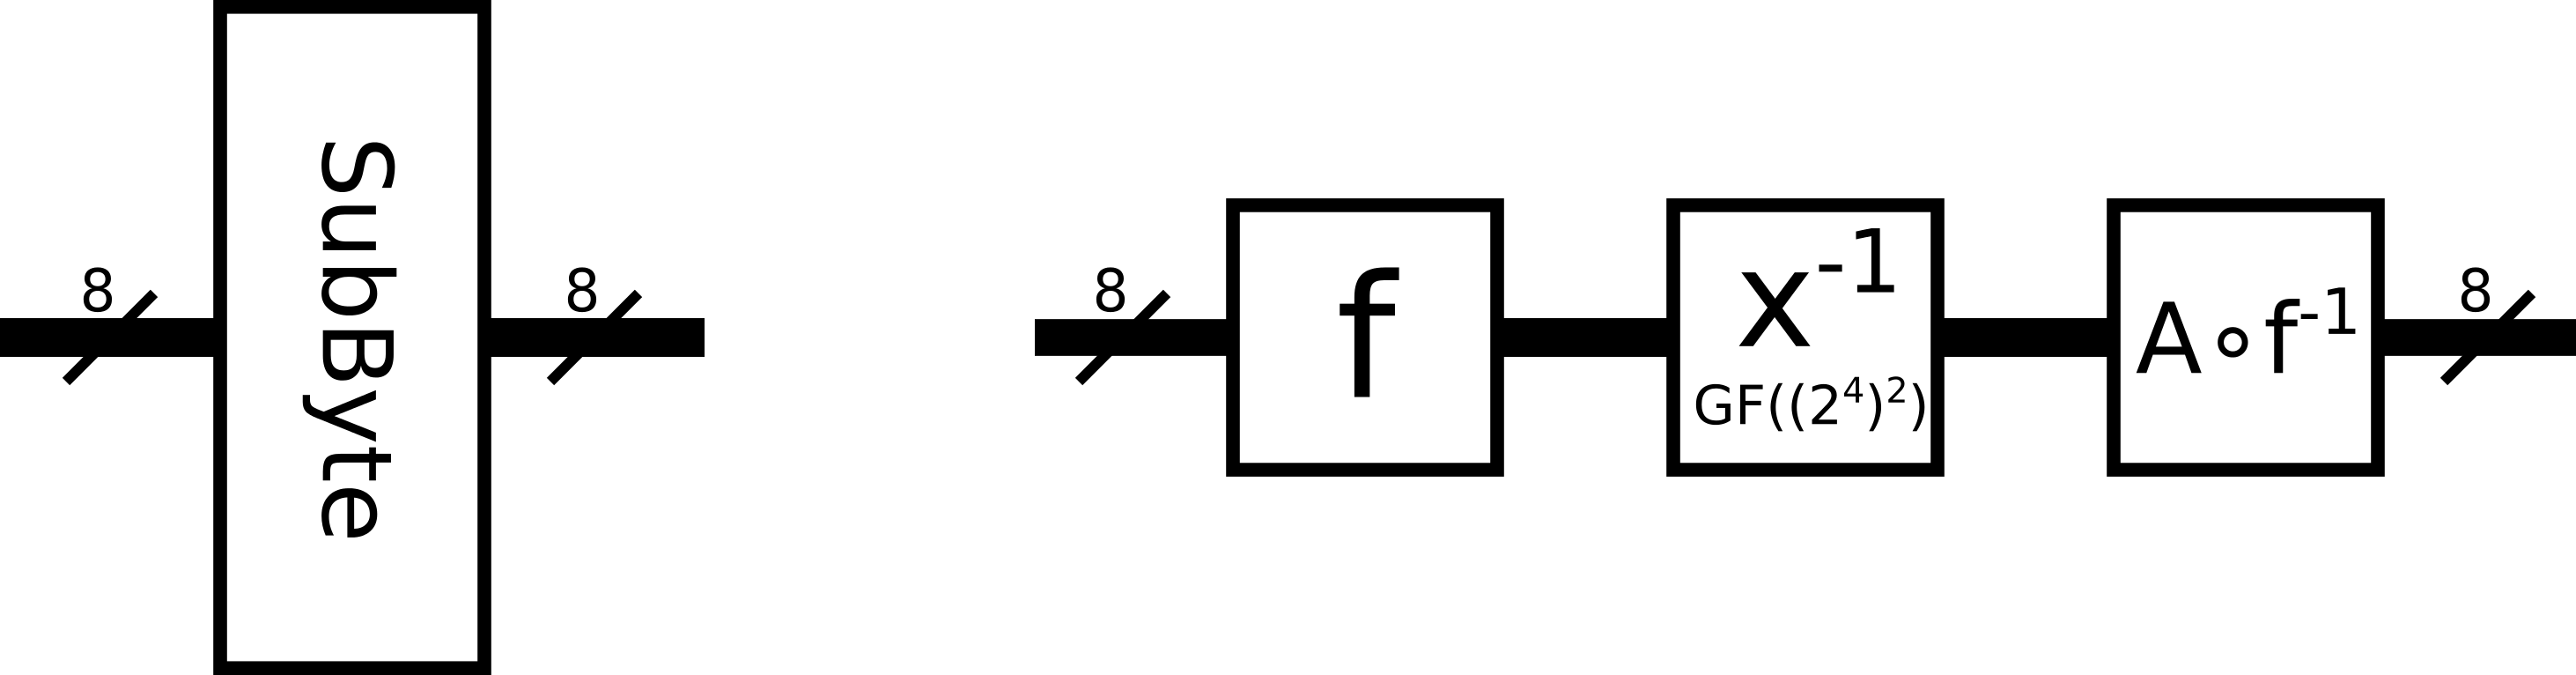
\includegraphics[scale=3]{sub-bytes}
\caption{SubButes transformation}
\end{figure}

Steps 3 and 4 can be joined into a single operation. SubBytes transformation for single byte can be implemented as a circuit in figure \ref{fig:sub-single-byte}. SubBytes transformation for entire state requires 16 such blocks. Detailed information about all required operations can be found in following paragraphs.

\paragraph{Composite Galois Fields and mapping between $GF(2^8)$ and $GF((2^4)^2)$}\mbox{}\\
We call two pairs
\begin{equation*}
\{GF(2^n), Q(y) = y^n + \sum_{i=0}^{n-1} q_i y^i, q_i \in GF(2) \}
\end{equation*}
\begin{equation*}
\{GF((2^n)^m), P(x) = x^m + \sum_{i=0}^{m-1} p_i x^i, p_i \in GF(2^n) \}
\end{equation*}
a composite field \cite{vlsi} if 
\begin{itemize}[nolistsep]
\item $GF(2^n)$ is constructed from $GF(2)$ by $Q(y)$
\item $GF((2^n)^m)$ is constructed from $GF(2^n)$ by $P(x)$
\end{itemize}
A composite field $GF((2^n)^m)$ is isomorphic to the field $GF(2^k)$ for $k = nm$ \cite{vlsi}.

For SubBytes transformation we will use the following composite fields and polynomials \cite{vlsi}:

\begin{equation}
\begin{aligned}
\label{eq:comp_fields_and_polys}
&GF(2) \Rightarrow GF(2^2) :               & P_0(x) = x^2 + x + 1\\
&GF(2^2) \Rightarrow GF((2^2)^2) :         & P_1(x) = x^2 + x + \phi\\
&GF((2^2)^2) \Rightarrow GF(((2^2)^2)^2) : & P_2(x) = x^2 + x + \lambda
\end{aligned}
\end{equation}

where $\phi = \{10\}$ and $\lambda = \{1100\}$.

An isomorphic mapping function $f(x)$ (\ref{eq:iso_map}) from $GF(2^8)$ to $GF((2^4)^2)$ can be found by exhaustive-search-based algorithm \cite{vlsi}. $\delta$ matrix corresponds to $p(x) = x^8 + x^4 + x^3 + x + 1$ (irreducible polynomial for $GF(2^8)$ defined in AES standard \cite{aes-standard}) and the polynomials in (\ref{eq:comp_fields_and_polys}). Reverse mapping from $GF((2^4)^2)$ to $GF(2^8)$ can be done with $f^{-1}(x)$ function (\ref{eq:iso_map_rev}).

\begin{equation}
\begin{gathered}
\label{eq:iso_map}
f(x) = \delta * x\\
x \in GF(2^8), f(x) \in GF((2^4)^2) \\
\begin{bmatrix}
b_0'\\b_1'\\b_2'\\b_3'\\b_4'\\b_5'\\b_6'\\b_7'
\end{bmatrix}
=
\begin{bmatrix}
    1 & 1 & 0 & 0 & 0 & 0 & 1 & 0 \\
    0 & 1 & 0 & 0 & 1 & 0 & 1 & 0 \\
    0 & 1 & 1 & 1 & 1 & 0 & 0 & 1 \\
    0 & 1 & 1 & 0 & 0 & 0 & 1 & 1 \\
    0 & 1 & 1 & 1 & 0 & 1 & 0 & 1 \\
    0 & 0 & 1 & 1 & 0 & 1 & 0 & 1 \\
    0 & 1 & 1 & 1 & 1 & 0 & 1 & 1 \\
    0 & 0 & 0 & 0 & 0 & 1 & 0 & 1
\end{bmatrix}
\begin{bmatrix}
b_0\\b_1\\b_2\\b_3\\b_4\\b_5\\b_6\\b_7
\end{bmatrix}
\end{gathered}
\end{equation}

\begin{equation}
\begin{gathered}
\label{eq:iso_map_rev}
f^{-1}(x) = \delta^{-1} * x\\
x \in GF((2^4)^2), f^{-1}(x) \in GF(2^8) \\
\begin{bmatrix}
b_0'\\b_1'\\b_2'\\b_3'\\b_4'\\b_5'\\b_6'\\b_7'
\end{bmatrix}
=
\begin{bmatrix}
    1 & 0 & 1 & 0 & 1 & 1 & 1 & 0 \\
    0 & 0 & 0 & 0 & 1 & 1 & 0 & 0 \\
    0 & 1 & 1 & 1 & 1 & 0 & 0 & 1 \\
    0 & 1 & 1 & 1 & 1 & 1 & 0 & 0 \\
    0 & 1 & 1 & 0 & 1 & 1 & 1 & 0 \\
    0 & 1 & 0 & 0 & 0 & 1 & 1 & 0 \\
    0 & 0 & 1 & 0 & 0 & 0 & 1 & 0 \\
    0 & 1 & 0 & 0 & 0 & 1 & 1 & 1
\end{bmatrix}
\begin{bmatrix}
b_0\\b_1\\b_2\\b_3\\b_4\\b_5\\b_6\\b_7
\end{bmatrix}
\end{gathered}
\end{equation}

A value $v = \{b_{2^n-1}...b_0\} \in GF((2^n)^2)$ is interpreted as a polynomial $p(x) = \sum_{i=0}^{n-1} b_ix^i$, where $b_i \in GF(2) = \{0, 1\}$ are bits. Any value $v \in GF((2^n)^2)$ can be represented as \cite{vlsi}:
\begin{equation}
\label{eq:poly_repr}
v = v_hx + v_l
\end{equation}
where $v_h = \{b_{2^n-1}...b_{2^{n-1}}\} \in GF(2^n)$ (high bits) and $v_l = \{b_{2^{n-1}-1}...b_0\} \in GF(2^n)$ (low bits). This holds true for decomposing values in $GF((2^n)^2)$ for any $n > 0$.

\paragraph{Affine transformation}\mbox{}\\
In SubBytes transformation, last step of calculating multiplicative inversion in $GF(2^8)$ is mapping $f^{-1}(x)$ from $GF((2^4)^2)$ to $GF(2^8)$. Immediately after this operation an affine transformation $a(x)$ is applied.
\begin{equation}
\begin{gathered}
\label{eq:affine}
a(x) = A * x + B\\
x \in GF(2^8), a(x) \in GF(2^8) \\
\begin{bmatrix}
b_0'\\b_1'\\b_2'\\b_3'\\b_4'\\b_5'\\b_6'\\b_7'
\end{bmatrix}
=
\begin{bmatrix}
    1 & 0 & 0 & 0 & 1 & 1 & 1 & 1 \\
    1 & 1 & 0 & 0 & 0 & 1 & 1 & 1 \\
    1 & 1 & 1 & 0 & 0 & 0 & 1 & 1 \\
    1 & 1 & 1 & 1 & 0 & 0 & 0 & 1 \\
    1 & 1 & 1 & 1 & 1 & 0 & 0 & 0 \\
    0 & 1 & 1 & 1 & 1 & 1 & 0 & 0 \\
    0 & 0 & 1 & 1 & 1 & 1 & 1 & 0 \\
    0 & 0 & 0 & 1 & 1 & 1 & 1 & 1
\end{bmatrix}
\begin{bmatrix}
b_0\\b_1\\b_2\\b_3\\b_4\\b_5\\b_6\\b_7
\end{bmatrix}
+
\begin{bmatrix}
1\\1\\0\\0\\0\\1\\1\\0
\end{bmatrix}
\end{gathered}
\end{equation}

As mapping $f^{-1}(x)$ from $GF((2^4)^2)$ to $GF(2^8)$ and affine transformation $a(x)$ are matrix multiplications, those two operations can be combined.
\begin{equation}
\begin{gathered}
\label{eq:affine}
f \circ a(x) = A * \delta * x + B\\
x \in GF(2^8), f \circ a(x) \in GF(2^8) \\
\begin{bmatrix}
b_0'\\b_1'\\b_2'\\b_3'\\b_4'\\b_5'\\b_6'\\b_7'
\end{bmatrix}
=
\begin{bmatrix}
    1 & 1 & 1 & 0 & 0 & 0 & 1 & 1 \\
    1 & 0 & 0 & 0 & 0 & 0 & 0 & 1 \\
    1 & 0 & 1 & 1 & 1 & 1 & 1 & 0 \\
    1 & 1 & 1 & 0 & 0 & 0 & 0 & 0 \\
    1 & 1 & 0 & 0 & 1 & 0 & 0 & 1 \\
    0 & 0 & 1 & 0 & 0 & 0 & 0 & 1 \\
    0 & 0 & 0 & 0 & 1 & 1 & 1 & 1 \\
    0 & 0 & 1 & 1 & 0 & 0 & 0 & 1
\end{bmatrix}
\begin{bmatrix}
b_0\\b_1\\b_2\\b_3\\b_4\\b_5\\b_6\\b_7
\end{bmatrix}
+
\begin{bmatrix}
1\\1\\0\\0\\0\\1\\1\\0
\end{bmatrix}
\end{gathered}
\end{equation}



\paragraph{Multiplicative inversion in $GF((2^4)^2)$}\mbox{}\\
In \cite{vlsi}[APPENDIX] it is proven that multiplicative inversion of $v = v_hx + v_l \in GF((2^4)^2)$ modulo $P_2(x)$ (\ref{eq:comp_fields_and_polys}) can be computed as in (\ref{eq:inv_formula_gf242}):
\begin{equation}
\begin{gathered}
\label{eq:inv_formula_gf242}
(v_hx + v_l)^{-1} = s_h \Theta x + (s_h + s_l) \Theta\\
\Theta = (s_h^2 \lambda + s_hs_l + s_l^2)^{-1} = (s_h^2 \lambda + s_l (s_h + s_l))^{-1}
\end{gathered}
\end{equation}

$\Theta$ and entire inversion can be implemented as circuits in figures \ref{fig:theta_impl} and \ref{fig:mul_inv_gf242}.

\begin{figure}
\label{fig:theta_impl}
\centering
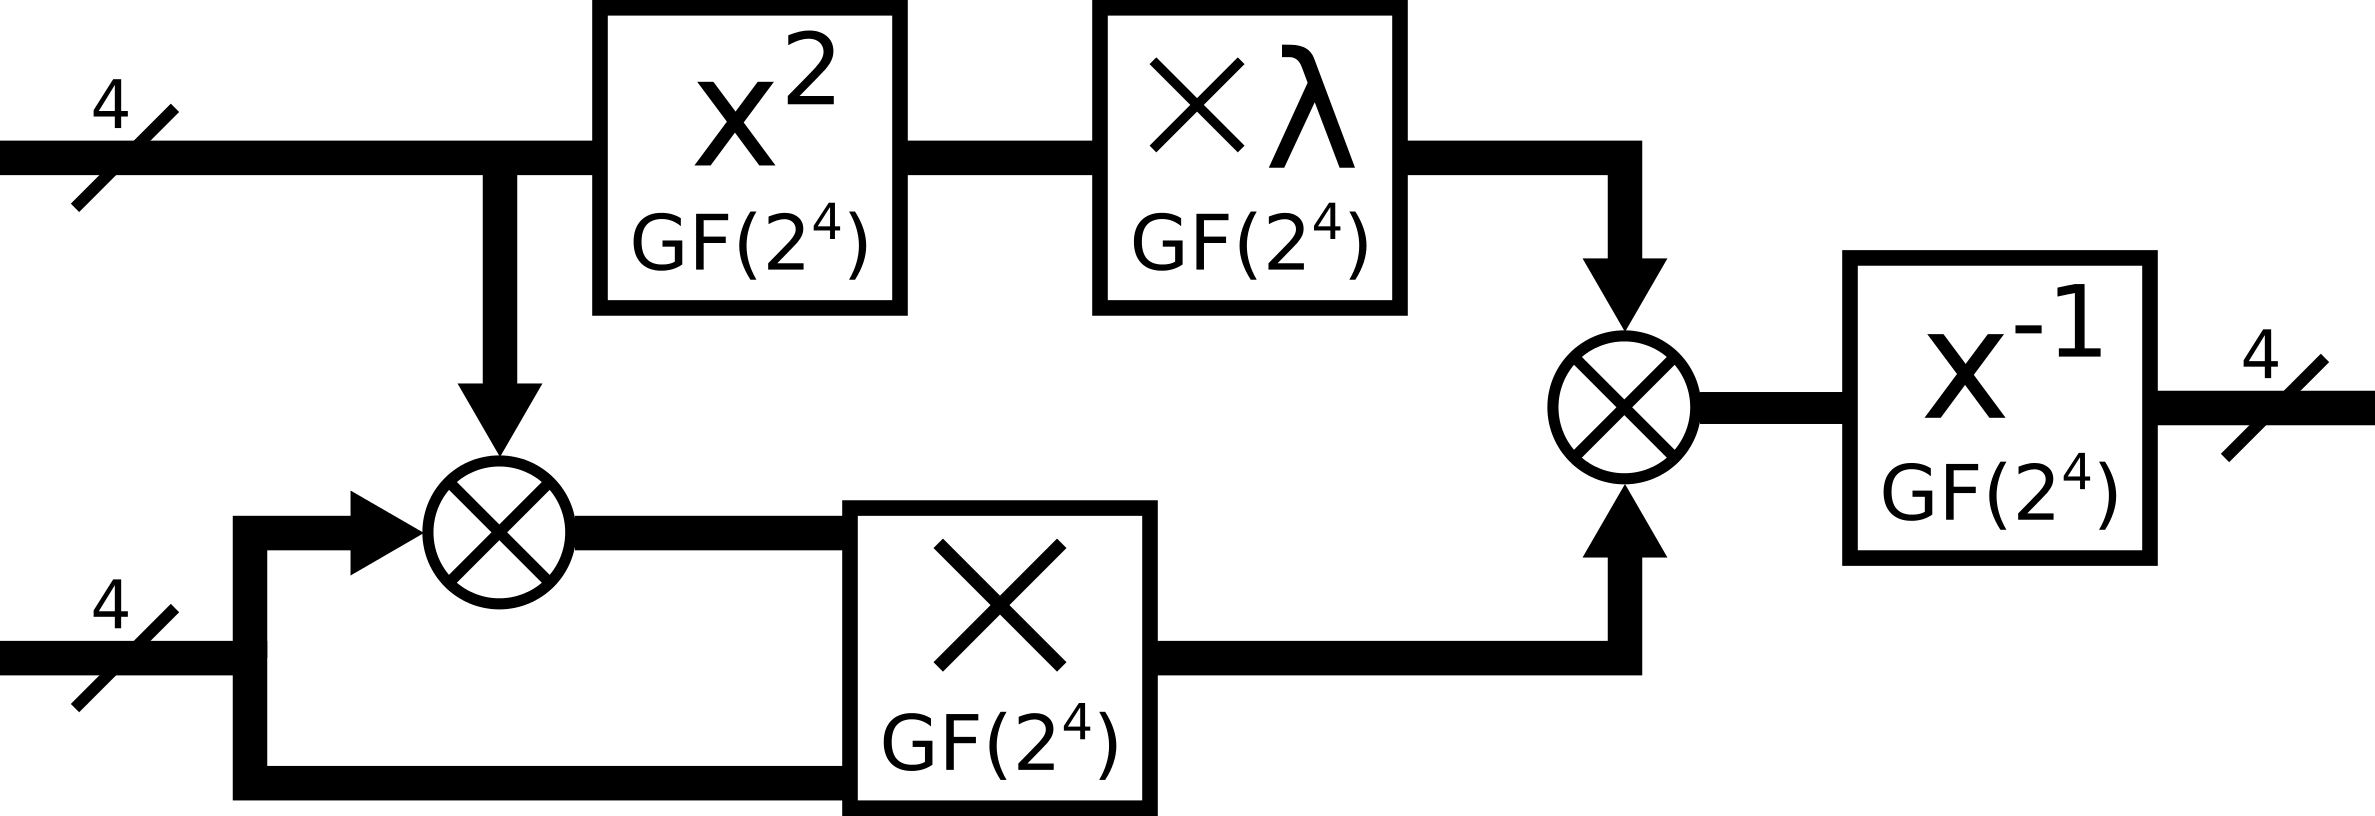
\includegraphics[scale=3]{theta-gf4}
\caption{Theta calculation circuit}
\end{figure}

\begin{figure}
\label{fig:mul_inv_gf242}
\centering
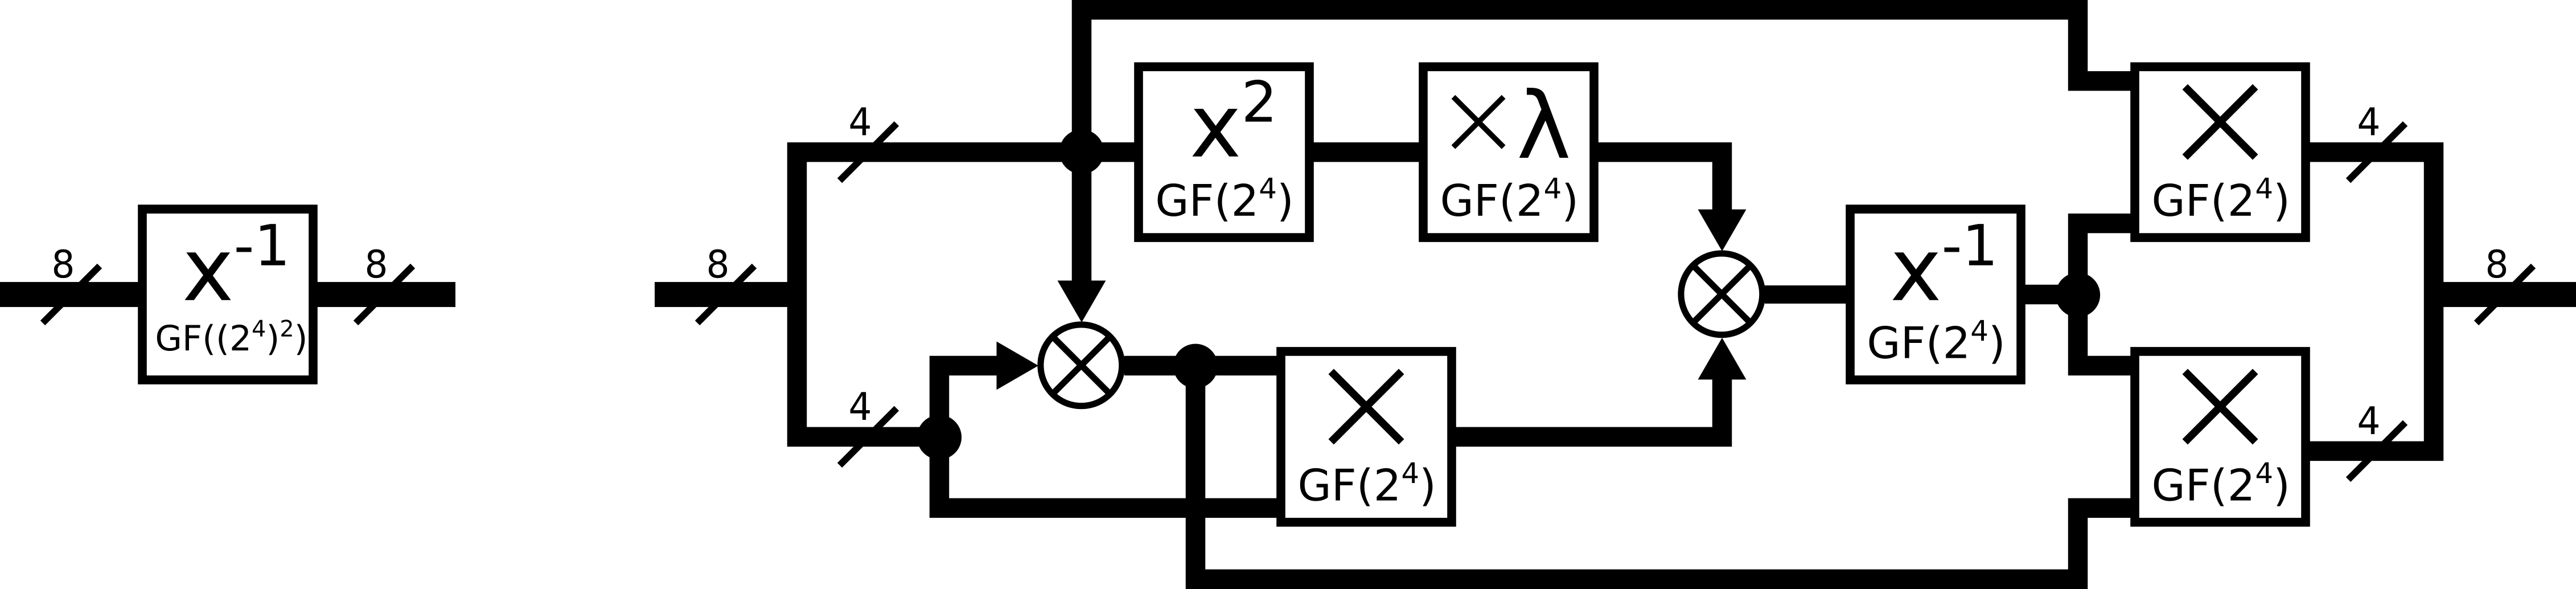
\includegraphics[scale=3]{inv-gf8}
\caption{Multiplicative inversion in $GF((2^4)^2)$ circuit}
\end{figure}

Operations to which multiplicative inversion in $GF((2^4)^2)$ is decomposed to are in $GF(2^4)$ and as a result the complecity of the solution is decreased. Some of those blocks are efficient to implement in hardware directly, and others can be decomposed even further.

\paragraph{Multiplicative inversion in $GF(2^4)$}\mbox{}\\
Authors of \cite{vlsi} derived that multiplicative inversion of $\{x_3x_2x_1x_0\} \in GF(2^4)$ can be calculated using formula (\ref{eq:mul_inf_gf24}).
\begin{equation}
\label{eq:mul_inf_gf24}
\begin{aligned}
x_3^{-1} &= x_3 + x_1x_2x_3 + x_0x_3 + x_2\\
x_2^{-1} &= x_1x_2x_3 + x_0x_2x_3 + x_0x_3 + x_2 + x_1x_2\\
x_1^{-1} &= x_3 + x_1x_2x_3 + x_0x_1x_3 + x_2 + x_0x_2 + x_1\\
x_0^{-1} &= x_1x_2x_3 + x_0x_2x_3 + x_1x_3 + x_0x_1x_3 + x_0x_3 + x_2 + x_1x_2 + x_0x_1x_2 + x_1 + x_0
\end{aligned}
\end{equation}

This can be further optimized for hardware implementation using substructure sharing (\ref{eq:mul_inf_gf24_opt}), which reduces the number of required operations to 9 multiplications ($and$ gates) and 14 additions ($xor$ gates).
\begin{equation}
\label{eq:mul_inf_gf24_opt}
\begin{aligned}
x_{01}   &= x_0x_1                             \\
x_{02}   &= x_0x_2                             \\
x_{03}   &= x_0x_3                             \\
x_{12}   &= x_1x_2                             \\
x_{13}   &= x_1x_3                             \\
x_{123}  &= x_{12}x_3                          \\
x_{023}  &= x_{02}x_3                          \\
x_{013}  &= x_{01}x_3                          \\
x_{012}  &= x_{01}x_2                          \\
a        &= x_{123} + x_2                      \\
b        &= a + x_{03}                         \\
c        &= x_{023} + x_{12}                   \\
d        &= x_{013} + x_{1}                    \\
x_3^{-1} &= b + x_3                            \\
x_2^{-1} &= b + c                              \\
x_1^{-1} &= a + d + x_3 + x_{02}               \\
x_0^{-1} &= b + c + d + x_{13} + x_{012} + x_0
\end{aligned}
\end{equation}


\begin{figure}
\label{fig:mul_inv_gf4_symbol}
\centering
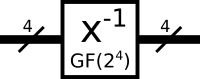
\includegraphics[scale=3]{inv-gf4-symbol}
\caption{Symbol of multiplicative inversion in $GF(2^4)$}
\end{figure}

In all diagrams symbol \ref{fig:mul_inv_gf4_symbol} will be used for multiplicative inversion in $GF(2^4)$


\paragraph{Multiplication by constant $\phi$ in $GF(2^2)$}\mbox{}\\
Lets first notice that for any $a \in GF(2^n)$ (\ref{eq:modulo_proof}) it is true. Keep in mind that coefficients of polynomials are in $GF(2^n)$ where addition is $xor$, so $(x + a) + (x + a) = 0$. This will be useful for decomposing operations between fields (\ref{eq:comp_fields_and_polys}) in deriving efficient circuits for them.
\begin{equation}
\label{eq:modulo_proof}
\begin{aligned}
x^2 &= (x^2 + x + a) + (x + a) &\\
x^2 &= (x + a)                 &\mod  x^2 + x + a
\end{aligned}
\end{equation}

As defined in (\ref{eq:comp_fields_and_polys}) \cite{vlsi} $\phi = \{10\}$. Product $k = \{k_1k_0\} \in GF(2^2)$ of $v = \{v_1v_0\} \in GF(2^2)$ by $\phi$ can be calculated as in \ref{eq:mul_phi}.

\begin{equation}
\label{eq:mul_phi}
\begin{aligned}
\phi v = x (v_1x + v_0) = v_1x^2 + v_0x &\stackrel{(\ref{eq:comp_fields_and_polys}, \ref{eq:modulo_proof})}{=} v_1(x + 1) + v_0x = (v_1 + v_0)x + v_1\\
k_1 &= v_1 + v_0\\
k_0 &= v_1
\end{aligned}
\end{equation}

It follows that multiplication by $\phi$ can be implemented as a circuit in fig. \ref{fig:phi_mul}.

\begin{figure}[!h]
\label{fig:phi_mul}
\centering
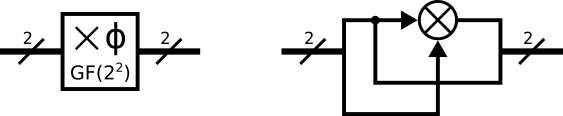
\includegraphics[scale=3]{mul-phi-gf2}
\caption{SubButes transformation decomposition}
\end{figure}


\paragraph{Multiplication by constant $\lambda$ in $GF(2^4)$}\mbox{}\\
As defined in (\ref{eq:comp_fields_and_polys}) \cite{vlsi} $\lambda = \{1100\} \in GF(2^4)$. Product $k = \{k_3k_2k_1k_0\} \in GF(2^4)$ of $v = \{v_3v_2v_1v_0\} \in GF(2^4)$ by $\lambda$ can be then calculated as in \ref{eq:mul_lambda}.

\begin{equation}
\label{eq:mul_lambda}
\begin{aligned}
\lambda v &= (\{11\}x) (\{v_3v_2\}x + \{v_1v_0\})\\
&= \{11\}\{v_3v_2\}x^2 + \{11\}\{v_1v_0\}x\\
&\stackrel{(\ref{eq:comp_fields_and_polys}, \ref{eq:modulo_proof})}{=}
\{11\}\{v_3v_2\}(x + \phi) + \{11\}\{v_1v_0\}x \\
&= (\{11\}\{v_3v_2\} + \{11\}\{v_1v_0\})x + \{11\}\{v_3v_2\}\phi\\
\{k_3k_2\} &= \{11\}\{v_3v_2\} + \{11\}\{v_1v_0\}\\
\{k_1k_0\} &= \{11\}\{v_3v_2\}\phi
\end{aligned}
\end{equation}

Multiplications of $\{v_1v_0\}$ and $\{v_3v_2\}$ by constant $\{11\}$ can be calculated similarly to multiplication by $\phi$ above (\ref{eq:mul_phi}).

\begin{equation}
\label{eq:mul_lambda_11}
\begin{aligned}
\{11\}\{v_bv_a\} &= (x + 1)(v_bx + v_a)\\
&= v_bx^2 + (v_b + v_a)x + v_a \\
&\stackrel{(\ref{eq:comp_fields_and_polys}, \ref{eq:modulo_proof})}{=}
v_b(x + 1) + (v_b + v_a)x + v_a \\
&= v_ax + (v_b + v_a)
\end{aligned}
\end{equation}

Combining (\ref{eq:mul_lambda}) and (\ref{eq:mul_lambda_11}) we can conclude (\ref{eq:mul_lambda2}).

\begin{equation}
\label{eq:mul_lambda2}
\begin{aligned}
\{k_3k_2\}
&\stackrel{(\ref{eq:mul_lambda_11})}{=}
(v_2x + (v_3 + v_2)) + (v_0x + (v_1 + v_0)) \\
&= (v_2 + v_0)x + (v_3 + v_2 + v_1 + v_0)\\
\{k_1k_0\}
&\stackrel{(\ref{eq:mul_lambda_11})}{=}
(v_2x + (v_3 + v_2))\phi \\
&\stackrel{(\ref{eq:mul_phi})}{=}
v_3x + v_2\\
k_3 &= v_2 + v_0\\
k_2 &= v_3 + v_2 + v_1 + v_0\\
k_1 &= v_3\\
k_0 &= v_2
\end{aligned}
\end{equation}


It follows that multiplication by $\lambda$ can be implemented as a circuit in fig. \ref{fig:lambda_mul}.

\begin{figure}[!h]
\label{fig:lambda_mul}
\centering
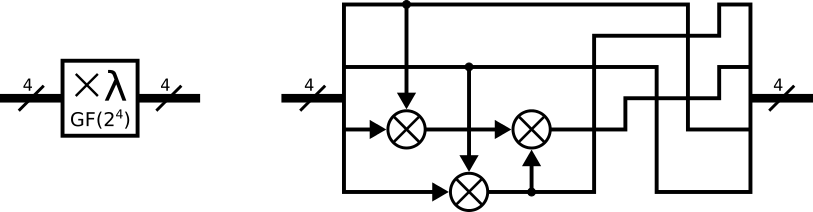
\includegraphics[scale=3]{mul-lam-gf4}
\caption{Constant multiplication by $\lambda$ circuit}
\end{figure}


\paragraph{Multiplication in $GF(2^2)$}\mbox{}\\
Product $k = \{k_1k_0\} \in GF(2^2)$ of $p = \{p_1p_0\} \in GF(2^2)$ by $q = \{q_1q_0\} \in GF(2^2)$ can be calculated as in (\ref{eq:mul_gf2}).

\begin{equation}
\label{eq:mul_gf2}
\begin{aligned}
pq &= (p_1x + p_0)(q_1x + q_0)\\
&= p_1q_1x^2 + (p_0q_1 + p_1q_0)x + p_0q_0\\
&\stackrel{(\ref{eq:comp_fields_and_polys}, \ref{eq:modulo_proof})}{=}
p_1q_1(x + 1) + (p_0q_1 + p_1q_0)x + p_0q_0\\
&=(p_1q_1 + p_0q_1 + p_1q_0)x + (p_1q_1 + p_0q_0)\\
k_1 &= p_1q_1 + p_0q_1 + p_1q_0\\
k_0 &= p_1q_1 + p_0q_0
\end{aligned}
\end{equation}

One can notice that for any $a, b, c, d \in GF(2^n)$ equation (\ref{eq:mul_gf_opt}) is always true.

\begin{equation}
\label{eq:mul_gf_opt}
\begin{aligned}
ad + bc + bd = (ac + ad + bc + bd) + ac = (a + b)(b + d) + ac
\end{aligned}
\end{equation}

To further reduce complexity of multiplication in $GF(2^2)$ by taking advantage of substructure sharing (of $p_0q_0$) and thus reducing overall number of used gates by 1, (\ref{eq:mul_gf_opt}) can be applied to (\ref{eq:mul_gf2}) ($a = p_0, b = p_1, c = q_0, d = q_1$).

\begin{equation}
\label{eq:mul_gf2_final}
\begin{aligned}
k_1 &= (p_0 + p_1)(q_0 + q_1) + p_0q_0\\
k_0 &= p_1q_1 + p_0q_0
\end{aligned}
\end{equation}


It follows that multiplication in $GF(2^2)$ (\ref{eq:mul_gf2_final}) can be implemented as a circuit in fig. \ref{fig:mul_gf2}.

\begin{figure}[!h]
\label{fig:mul_gf2}
\centering
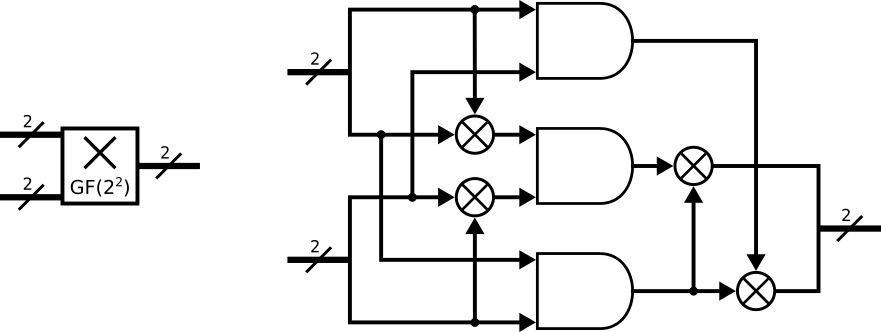
\includegraphics[scale=3]{mul-gf2}
\caption{Multiplication in $GF(2^2)$ circuit}
\end{figure}



\paragraph{Multiplication in $GF(2^4)$}\mbox{}\\
Product $k = \{k_3k_2k_1k_0\} \in GF(2^4)$ of $p = \{p_3p_2p_1p_0\} \in GF(2^4)$ by $q = \{q_3q_2q_1q_0\} \in GF(2^4)$ can be calculated as in (\ref{eq:mul_gf4}).

\begin{equation}
\label{eq:mul_gf4}
\begin{aligned}
pq &= (\{p_3p_2\}x + \{p_1p_0\})(\{q_3q_2\}x + \{q_1q_0\})\\
&= \{p_3p_2\}\{q_3q_2\}x^2 + (\{p_1p_0\}\{q_3q_2\} + \{p_3p_2\}\{q_1q_0\})x + \{p_1p_0\}\{q_1q_0\} \\
&\stackrel{(\ref{eq:comp_fields_and_polys}, \ref{eq:modulo_proof})}{=}
\{p_3p_2\}\{q_3q_2\}(x + \phi) + (\{p_1p_0\}\{q_3q_2\} + \{p_3p_2\}\{q_1q_0\})x + \{p_1p_0\}\{q_1q_0\} \\
&= (\{p_3p_2\}\{q_3q_2\} + \{p_1p_0\}\{q_3q_2\} + \{p_3p_2\}\{q_1q_0\})x + (\{p_3p_2\}\{q_3q_2\}\phi + \{p_1p_0\}\{q_1q_0\})\\
\{k_3k_2\} &= \{p_3p_2\}\{q_3q_2\} + \{p_1p_0\}\{q_3q_2\} + \{p_3p_2\}\{q_1q_0\}\\
\{k_1k_0\} &= \{p_3p_2\}\{q_3q_2\}\phi + \{p_1p_0\}\{q_1q_0\}
\end{aligned}
\end{equation}

To further reduce complexity of multiplication in $GF(2^4)$ by reducing number of $GF(2^2)$ multiplications (\ref{eq:mul_gf_opt}) can be applied to (\ref{eq:mul_gf4}) ($a = \{p_1p_0\}, b = \{p_3p_2\}, c = \{q_1q_0\}, d = \{q_3q_2\}$).

\begin{equation}
\label{eq:mul_gf4_final}
\begin{aligned}
\{k_3k_2\} &= (\{p_1p_0\} + \{p_3p_2\})(\{q_1q_0\} + \{q_3q_2\}) + \{p_1p_0\}\{q_1q_0\}\\
\{k_1k_0\} &= \{p_3p_2\}\{q_3q_2\}\phi + \{p_1p_0\}\{q_1q_0\}
\end{aligned}
\end{equation}



It follows that multiplication in $GF(2^4)$ can be implemented as a circuit in fig. \ref{fig:mul_gf4}.

\begin{figure}[!h]
\label{fig:mul_gf4}
\centering
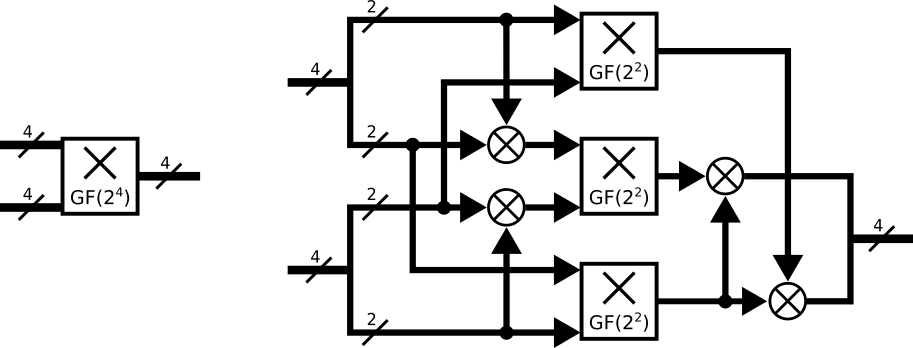
\includegraphics[scale=3]{mul-gf4}
\caption{Multiplication in $GF(2^4)$ circuit}
\end{figure}


\paragraph{Squaring in $GF(2^4)$}\mbox{}\\
Lets first establish how squaring in $GF(2^2)$ can be calculated. 
Square $s = \{s_1s_0\} \in GF(2^2)$ of $d = \{d_1d_0\} \in GF(2^2)$ can be calculated as in \ref{eq:gq_gf2}. Keep in mind that squating in $GF(2)$ is an $and$ operation and thus for any $l \in GF(2)$ it is true that $l^2 = l$.

\begin{equation}
\label{eq:sq_gf2}
\begin{aligned}
s^2 &= (d_1x + d_0)(d_1x + d_0) \\
&= d_1^2x^2 + (d_1d_0 + d_1d_0)x + d_0^2 \\
&= d_1^2x^2 + d_0^2 \\
&= d_1x^2 + d_0\\
&\stackrel{(\ref{eq:comp_fields_and_polys}, \ref{eq:modulo_proof})}{=}
d_1(x + 1) + d_0 \\
&= d_1x + (d_1 + d_0)\\
s_1 &= d_1\\
s_0 &= d_1 + d_0
\end{aligned}
\end{equation}

Square $k = \{k_3k_2k_1k_0\} \in GF(2^4)$ of $v = \{v_3v_2v_1v_0\} \in GF(2^4)$ can be calculated as in \ref{eq:sq_gf4}.

\begin{equation}
\label{eq:sq_gf4}
\begin{aligned}
k^2 &= (\{v_3v_2\}x + \{v_1v_0\})(\{v_3v_2\}x + \{v_1v_0\})\\
&= \{v_3v_2\}^2x^2 + (\{v_3v_2\}\{v_1v_0\} + \{v_3v_2\}\{v_1v_0\})x + \{v_1v_0\}^2 \\
&= \{v_3v_2\}^2x^2 + \{v_1v_0\}^2 \\
&\stackrel{(\ref{eq:comp_fields_and_polys}, \ref{eq:modulo_proof})}{=}
\{v_3v_2\}^2(x + \phi) + \{v_1v_0\}^2 \\
&= \{v_3v_2\}^2x + (\{v_1v_0\}^2 + \{v_3v_2\}^2\phi)\\
\{k_3k_2\} &= \{v_3v_2\}^2 \\
\{k_1k_0\} &= \{v_1v_0\}^2 + \{v_3v_2\}^2\phi
\end{aligned}
\end{equation}

Applying (\ref{eq:sq_gf2}) to (\ref{eq:sq_gf4}) yields final formula (\ref{eq:sq_gf4_final}), which can be implemented in hardware as a circuit \ref{fig:sq_sq4}.
\begin{equation}
\label{eq:sq_gf4_final}
\begin{aligned}
\{k_3k_2\} &= \{v_3v_2\}^2 = (v_3x + v_2)^2
\stackrel{(\ref{eq:sq_gf2})}{=}
v_3x + (v_3 + v_2)\\
\{k_1k_0\} &= \{v_1v_0\}^2 + \{v_3v_2\}^2\phi \\
&= (v_1x + v_0)^2 + (v_3x + v_2)^2\phi \\
&\stackrel{(\ref{eq:sq_gf2})}{=}
(v_1x + (v_1 + v_0)) + (v_3x + (v_3 + v_2))\phi \\
&\stackrel{(\ref{eq:mul_phi})}{=}
(v_1x + (v_1 + v_0)) + (v_2x + v_3)) \\
&= (v_2 + v_1)x + (v_3 + v_1 + v_0) \\
k_3 &= v_3 \\
k_2 &= v_3 + v_2 \\
k_1 &= v_2 + v_1 \\
k_0 &= v_3 + v_1 + v_0
\end{aligned}
\end{equation}

\begin{figure}[!h]
\label{fig:mul_sq4}
\centering
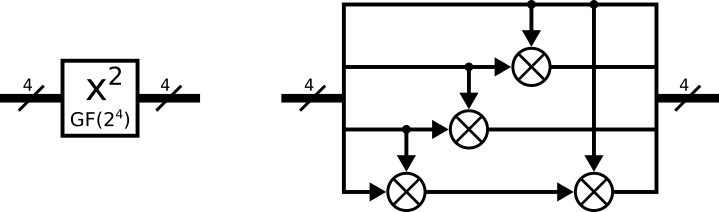
\includegraphics[scale=3]{sq-gf4}
\caption{Squaring in $GF(2^4)$ circuit}
\end{figure}

\subsection{MixColumns transformation}

MixColumns transformation is most efficient to be implemented directly in $GF(2^8)$. Unlike in SubBytes transformation, all attempts to decompose operations lead to increase of overall number of required logic gates. This is because \cite{vlsi}:

\begin{itemize}[nolistsep]
\item mapping values to and from composite fields requires additional logic
\item constants used in MixColumns have less non-zero bits in $GF(2^8)$ ($\{02\}_{16}$, $\{03\}_{16}$) than in $GF((2^2)^4)$ ($\{5f\}_{16}$, $\{5e\}_{16}$), which results in more logic gates required to perform multiplication by them.
\end{itemize}

MixColumns transformation can be efficiently implemented by taking advantage of substructure sharing. Lets first notice that multiplying any $a \in GF(2^8)$ by $\{03\}_{16}$ can be substituted by multiplication by $\{02\}_{16}$ and one addition:

\begin{equation}
\label{eq:decomp_mul_3}
\{03\}_{16}a = (x + 1)a = ax + a = \{02\}_{16}a + a
\end{equation}

Taking that into consideration we can derive equations for MixColums transformation:

\begin{equation}
\label{xd}
\begin{aligned}
B_0' &= \{02\}_{16}B_0 + \{03\}_{16}B_1 + B_2 + B_3 \\
&\stackrel{(\ref{eq:decomp_mul_3})}{=}
\{02\}_{16}B_0 + (\{02\}_{16}B_1 + B_1) + B_2 + B_3 \\
&= \{02\}_{16}(B_0 + B_1) + (B_2 + B_3) + B_1 \\ \\
%
B_1' &= B_0 + \{02\}_{16}B_1 + \{03\}_{16}B_2 +  B_3 \\ 
&\stackrel{(\ref{eq:decomp_mul_3})}{=}
B_0 + (\{02\}_{16}B_1 + B_1) + \{02\}_{16}B_2 + B_3 \\ 
&= \{02\}_{16}(B_1 + B_2) + (B_0 + B_3) + B_2\\ \\
%
B_2' &= B_0 + B_1 + \{02\}_{16}B_2 + \{03\}_{16}B_3 \\
&\stackrel{(\ref{eq:decomp_mul_3})}{=}
B_0 + B_1 + \{02\}_{16}B_2 + (\{02\}_{16}B_3 + B_3) \\
&= \{02\}_{16}(B_2 + B_3) + (B_0 + B_1) + B_3 \\ \\
%
B_3' &= \{03\}_{16}B_0 + B_1 + B_2 + \{02\}_{16}B_3 \\
&\stackrel{(\ref{eq:decomp_mul_3})}{=}
(\{02\}_{16}B_0 + B_0) + B_1 + B_2 + \{02\}_{16}B_3 \\
&= \{02\}_{16}(B_0 + B_3) + (B_1 + B_2) + B_0
\end{aligned}
\end{equation}

where $B_i$ are AES bytes, $[B_0, B_1, B_2, B_3]$ is input column and $[B_0', B_1', B_2', B_3']$ is transformed column. MixColumns transformation for a single column can be therefore implemented as shown in figure \ref{fig:mix_columns}. MixColumns transformation on entire AES state consists of 4 such circuits.

\begin{figure}[!h]
\label{fig:mix_columns}

\centering
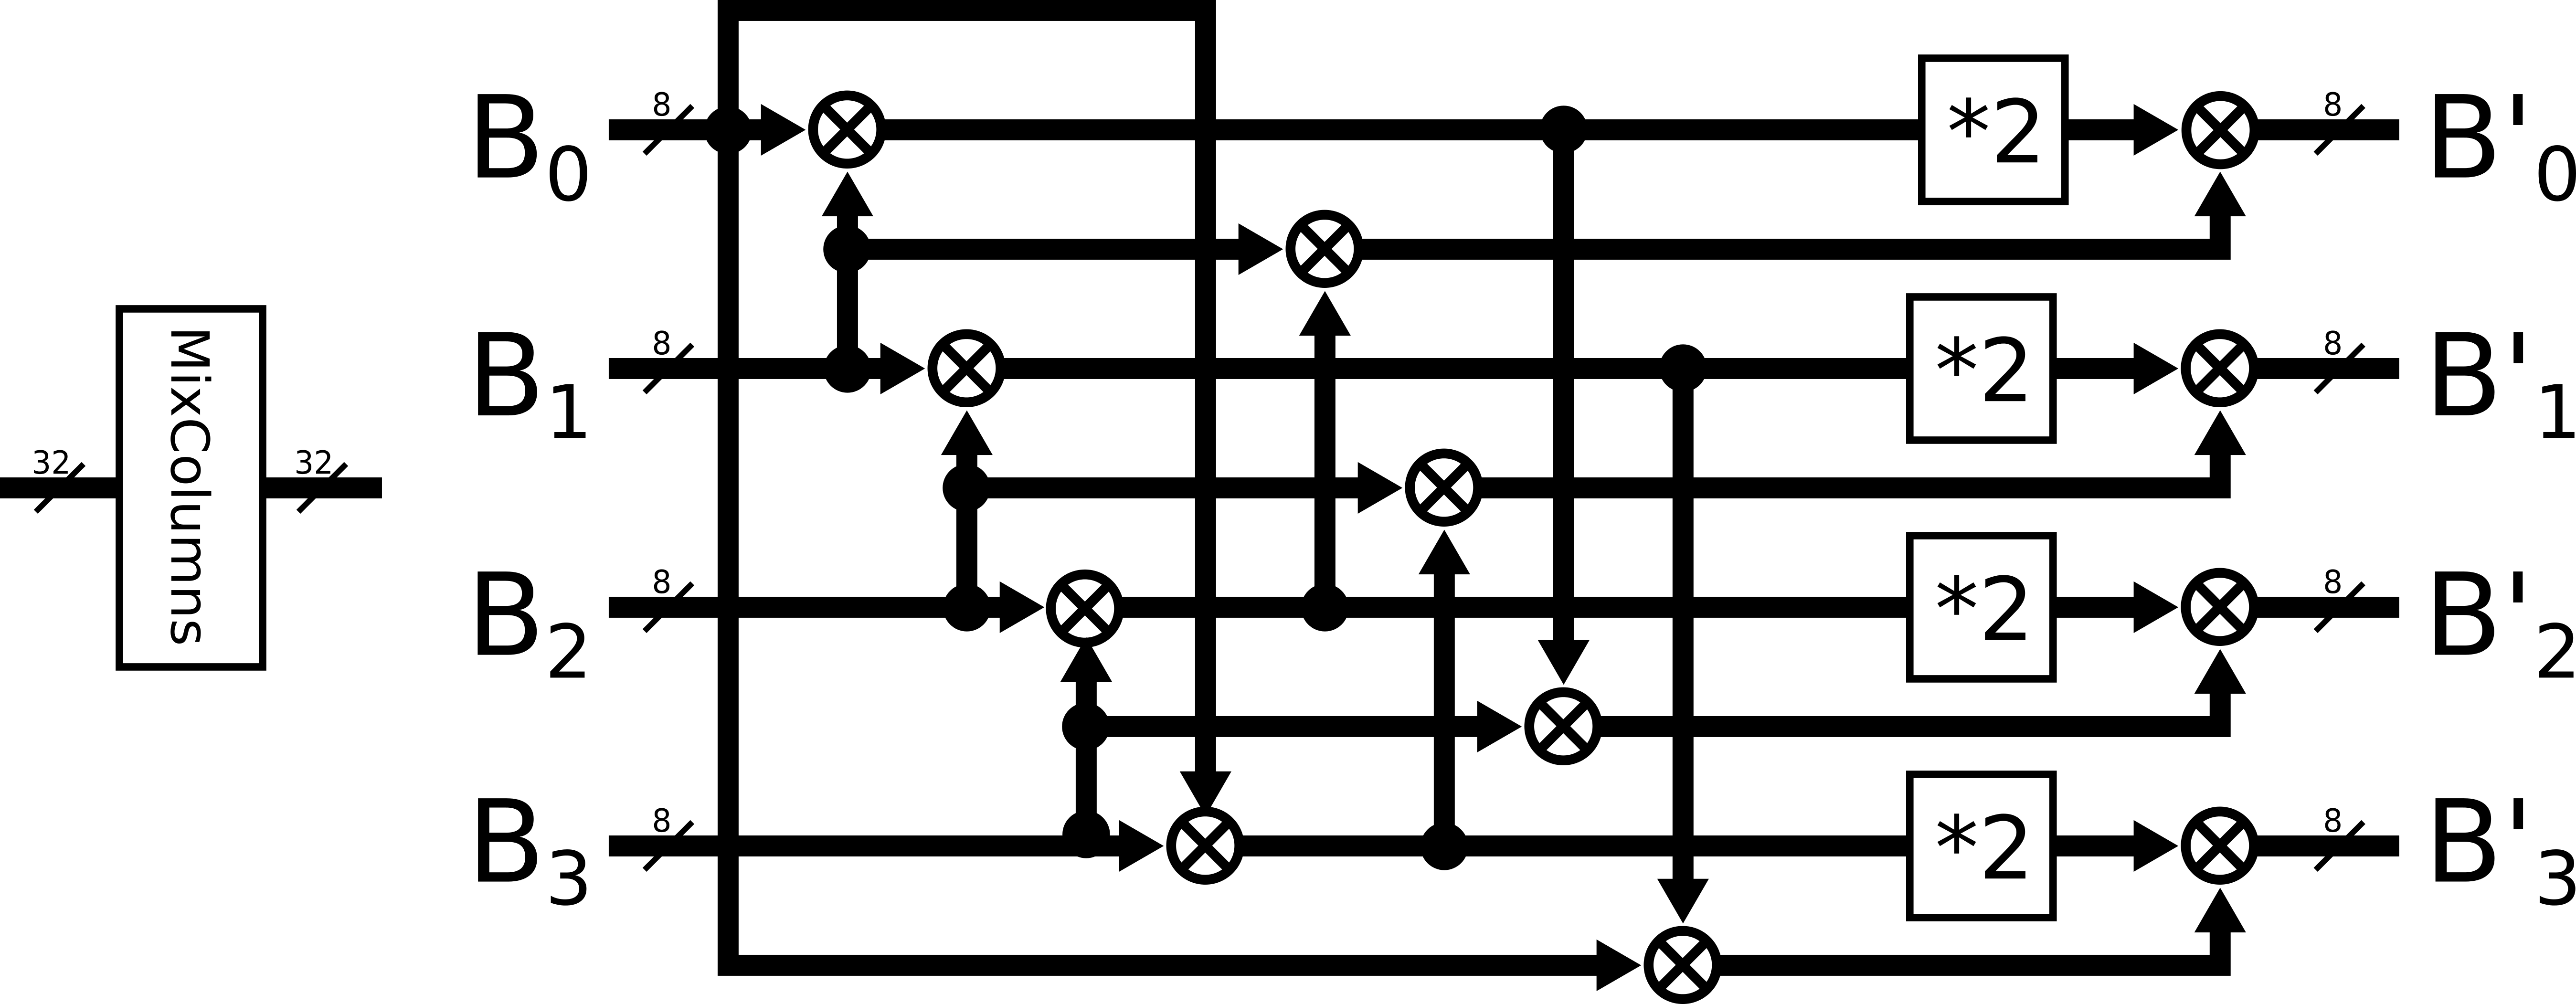
\includegraphics[scale=2.5]{mix-columns}

\caption{MixColumns transformation circuit}
\end{figure}

Multiplication by $\{02\}_{16}$ can be calculated according to formula (\ref{eq:mul2}) \cite{vlsi}: 

\begin{equation}
\label{eq:mul2}
\{02\}_{16}S = xS = s_6x^7 + s_5x^6 + s_4x^5 + (s_3 + s_7)x^4 + (s_2 + s_7)x^3 + s_1x^2 + (s_0 + s_7)x + s_7
\end{equation}

which requires 3 $xor$ gates.



\subsection{AddRoundKey transformation}

AddRoundKey is a transformation that adds (xor) round key to AES state. Round keys are obtained using key expansion routine, which is defined in AES enctroption standard \cite{aes-standard}. Expansion algorithm performs byte substitution on some bytes similarly to SubBytes transformation, therefore it can be implemented in two ways as well:

\begin{itemize}[nolistsep]
\item Using a look-up table of precomputed values stored in on-chip memory
\item Using only combinatorial logic.
\end{itemize}

Advantages and disadvantages of both appraches are same as for SubBytes transformation. This section will describe KeyExpansion circuit based on operations already defined in section \ref{sec:sub-bytes}.

To calculate round key for round $N$, key for round $N - 2$ is used. In order to be able to construct efficient pipelie, key expansion for each round needs to be calculated 2 rounds ahead of time. To perform expansion of key for round $N + 2$ circuit in figure \ref{fig:key-expansion} can be used. Such circuit would be placed in final pipelined design concurrent to round $N$. Note that key for round $N + 1$ is not used in calculation and is forwarded to next pipeline stage unmodified.

Key schedule for first round is 128 highest bits of AES key provided by user. For second round 128 lowest bits of AES key are used. For subsequent rounds key schedules are calculated according to AES key expansion algorithm (\cite{aes-standard}).

\begin{figure}[!h]
\centering
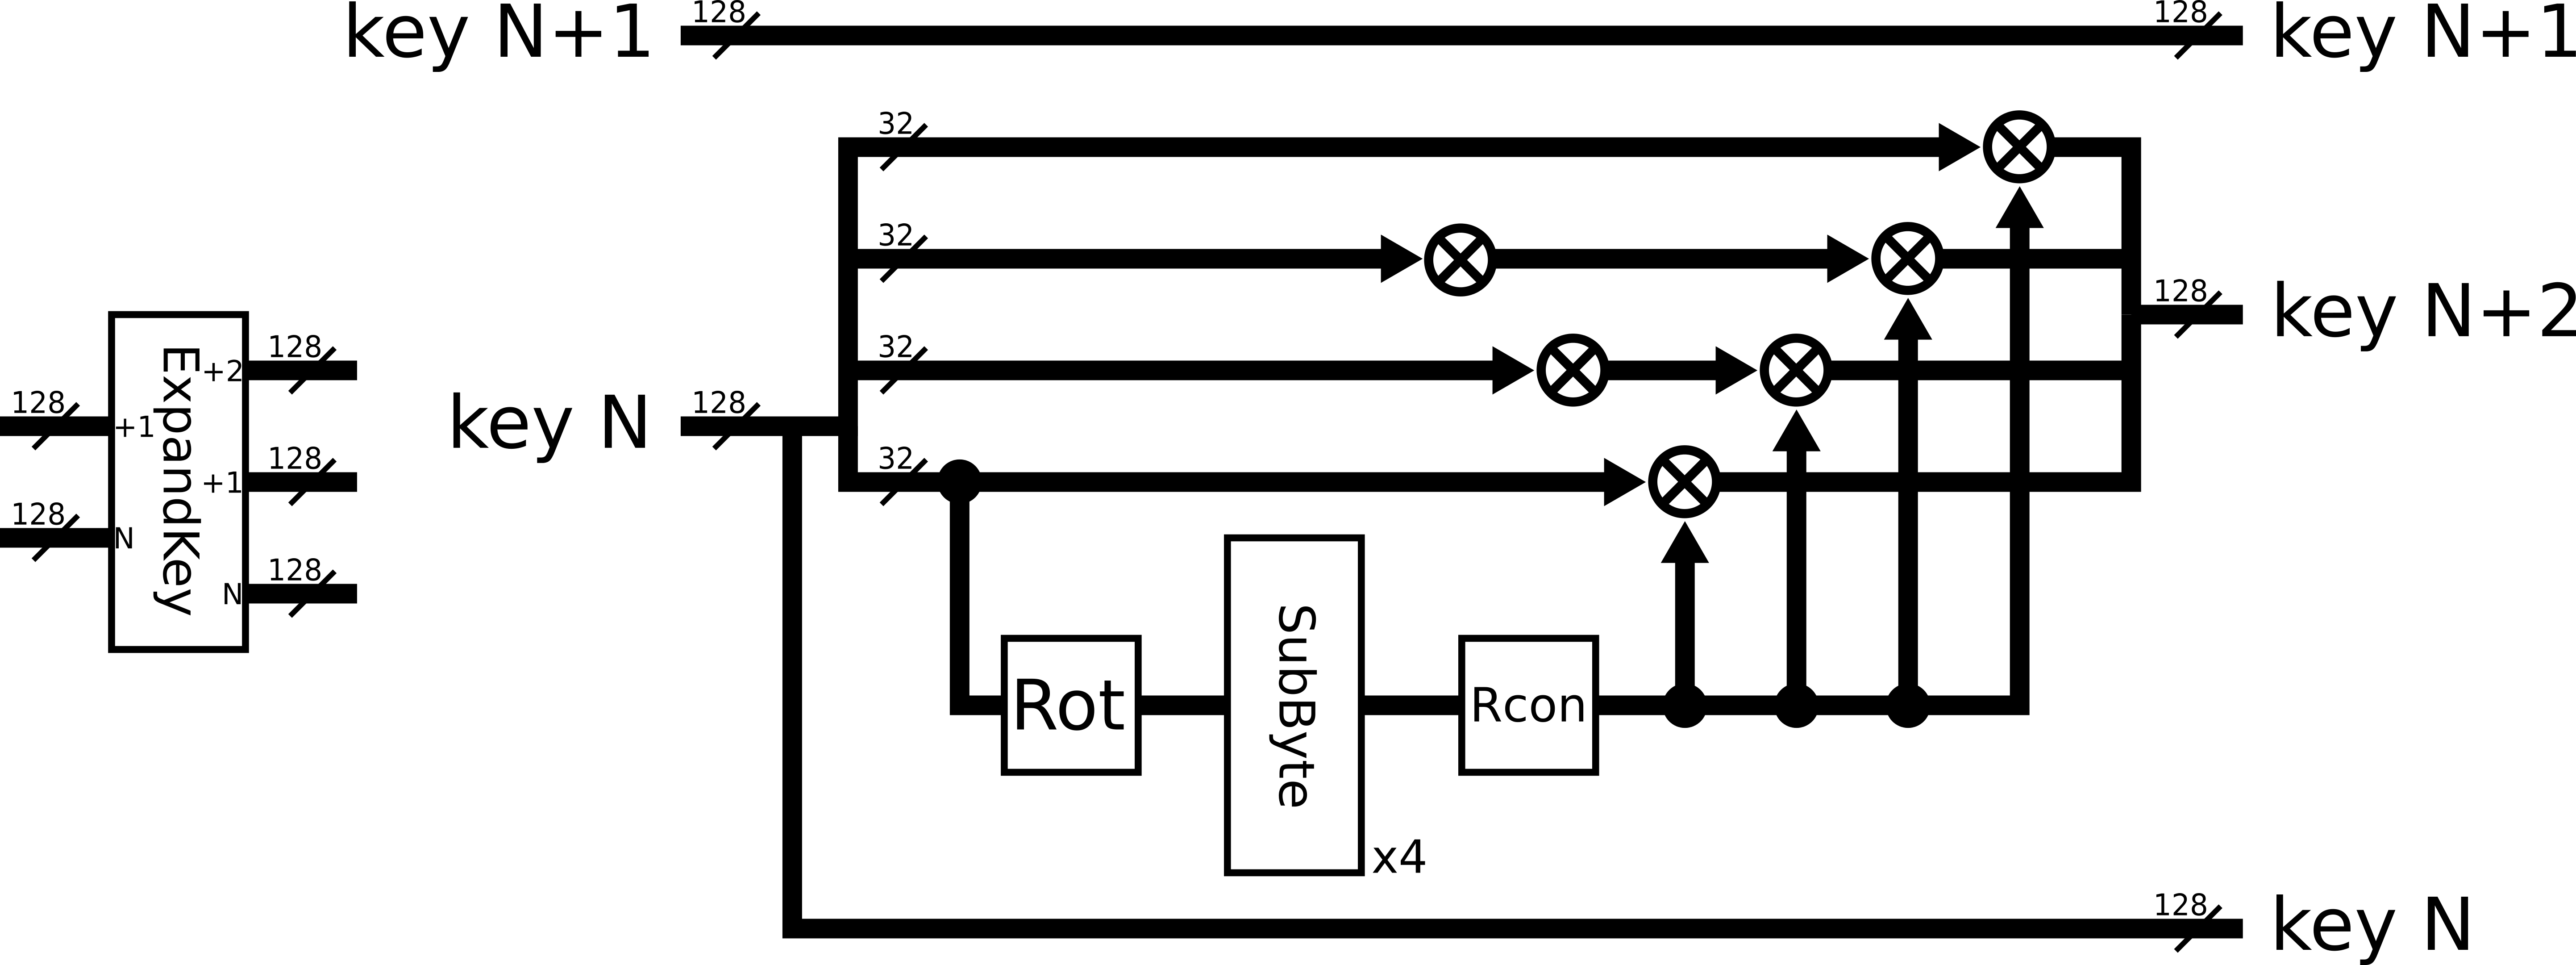
\includegraphics[scale=2.8]{key-expansion}
\caption{Key expansion circuit}
\label{fig:key-expansion}
\end{figure}

Operation $Rot$ rotates a word (4 bytes) left by one byte, and $Rcon$ xors highest byte of a word with $2^{N + 1}$. Those operation are only applied in rounds $N$, where $N \equiv 1 \pmod{2}$.


\subsection{ShiftRows transformation}

ShiftRows transformation does not use any combinatorial logic, it only rearranges order of bits in AES state. As a consequence it does not use any FPGA logic resources and only requires adequate routing.

\begin{figure}[!h]
\centering
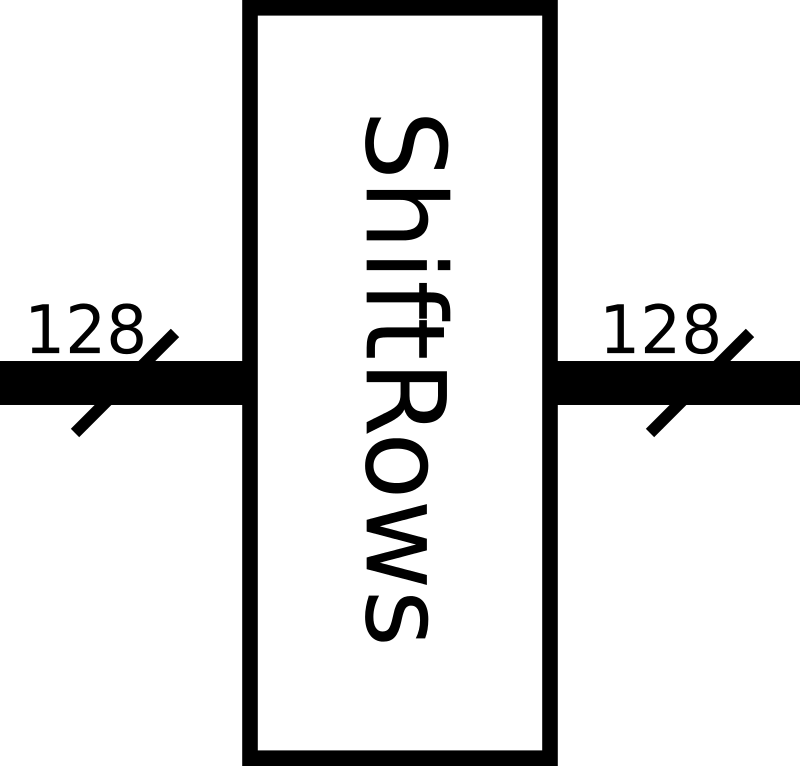
\includegraphics[scale=4]{shift-rows}
\caption{ShiftRows transformation symbol}
\label{fig:shift-rows}
\end{figure}
\subsection{AES encryption round}

AES Encryption rounds consist of four transformations explained in previous section. A circuit that can be used to implement a round is presented in figure \ref{fig:aes-round}.

\begin{figure}[!h]
\centering
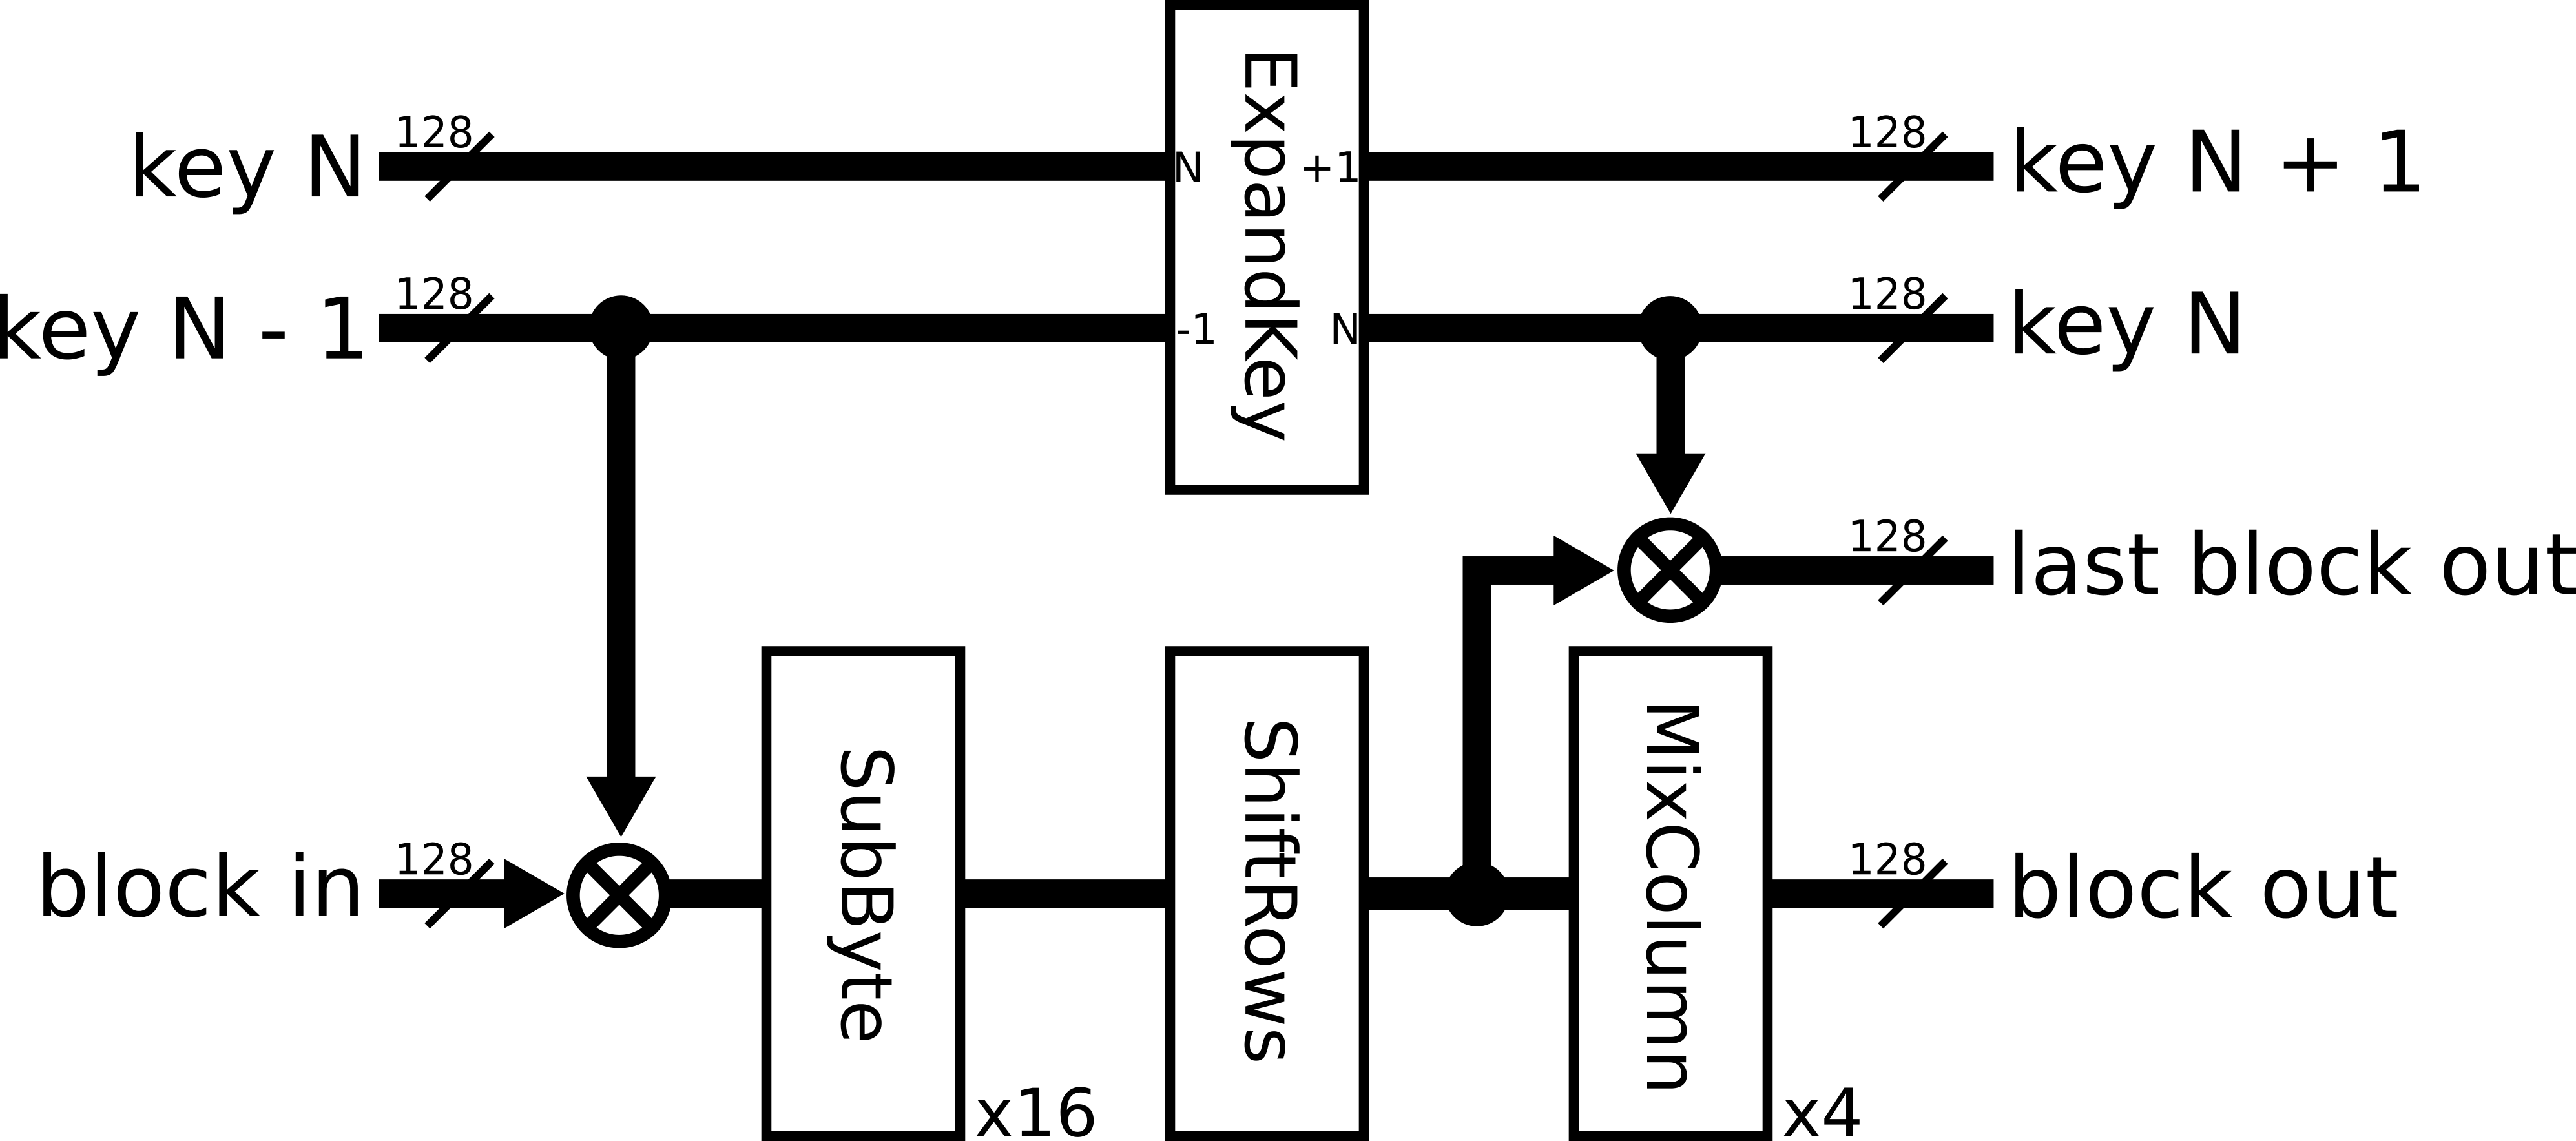
\includegraphics[scale=4]{aes-round}
\caption{AES round circuit}
\label{fig:aes-round}
\end{figure}

256-bit version of AES encryption algorith, which is analysed here, has 15 rounds. Rounds 2 to 14 are the same and use all four transformations (fig. \ref{fig:aes-round}). First round only applies AddRoundKey transformation to the state. Last round is similar to rounds 2 to 14, but it does not apply MixColumns transformation.



\section{Testing methodology}
\label{sec:testing-methodology}

\subsection{Throughput}
To determine throughput of design components a testing circuit was developed and implemented in FPGA. This approach was the only feasible way to perform this measurement as FPGA chip on the Altera DE1 SoC Developement Board is not connected to any interfaces that are fast enough to keep up with the speed of implemented encryption module. This is only a limitation of the development board that was used and not FPGA technology itself. It could be overcome by choosing or designing a circuit board that provides sufficiently fast interfaces, for example PCI Express 3.0 16x.

Throughput was determined by measuring frequency at which the design can operate without errors for extended period of time, and then multiplying it by AES block size (128b). Maximum frequency was looked for by:
\begin{enumerate}[nolistsep]
\item Changing design parameters to reflect desired frequency - PLL multipliers and timing constraints.
\item Recompiling the design in \textit{High Effort - Max Performance} mode - to ensure that updated design is placed optimally for given frequency.
\item Deploying the design to FPGA and running it for at least 30 minutes, or until first error occurance.
\end{enumerate}
A design was considered stable at given frequency when it could operate without any errors for at least 30 minutes. Maximum stable frequency was looked for using binary search in range $[100MHz - 600MHz]$. 

To make sure that no unrealistic optimizations were made during compilation and placement, input and expected blocks were not hardcoded into the design, but rather placed in on-chip ROM. This approach also resulted in more realistic placement environment for the encryption module - input and output signals had to be routed to ROM blocks. This required additional routing, as would exposing those signals to FPGA pins. 

Using ROM as storage for testing data introduced a limitation of 315MHz frequency, which is the highest frequency at which on-chip ROM can operate \cite[Table 2-1]{altera-vol1} . This was a problem, because expected maximum frequency of AES encryption was above 315MHz. This limitation, hovewer, can be overcome. Two different designs were considered, both were capable of testing circuits at very similar maximum frequencies (over 500MHz). Approach based on multiplexing two streams of blocks was both simpler (required less logic elements) and capable of operating at slightly higher frequency (530MHz), and it was chosen to be used in testing.


\subsubsection{Multiplexer based memory solution}
This approach uses two alternating banks of ROM (fig. \ref{fig:memory-arrangement}), both 128 bits wide (AES block size) and 32 blocks deep (contain 32 blocks). Each bank reads data from memory in two cycles of main clock (enable signal is used to divide the clock by 2). Streams of blocks from the two ROM banks are multiplexed together to form a single stream of testing data. Using this method for delivering data blocks to test module allows for operation at 530MHz. 

\begin{figure}[!h]
\centering
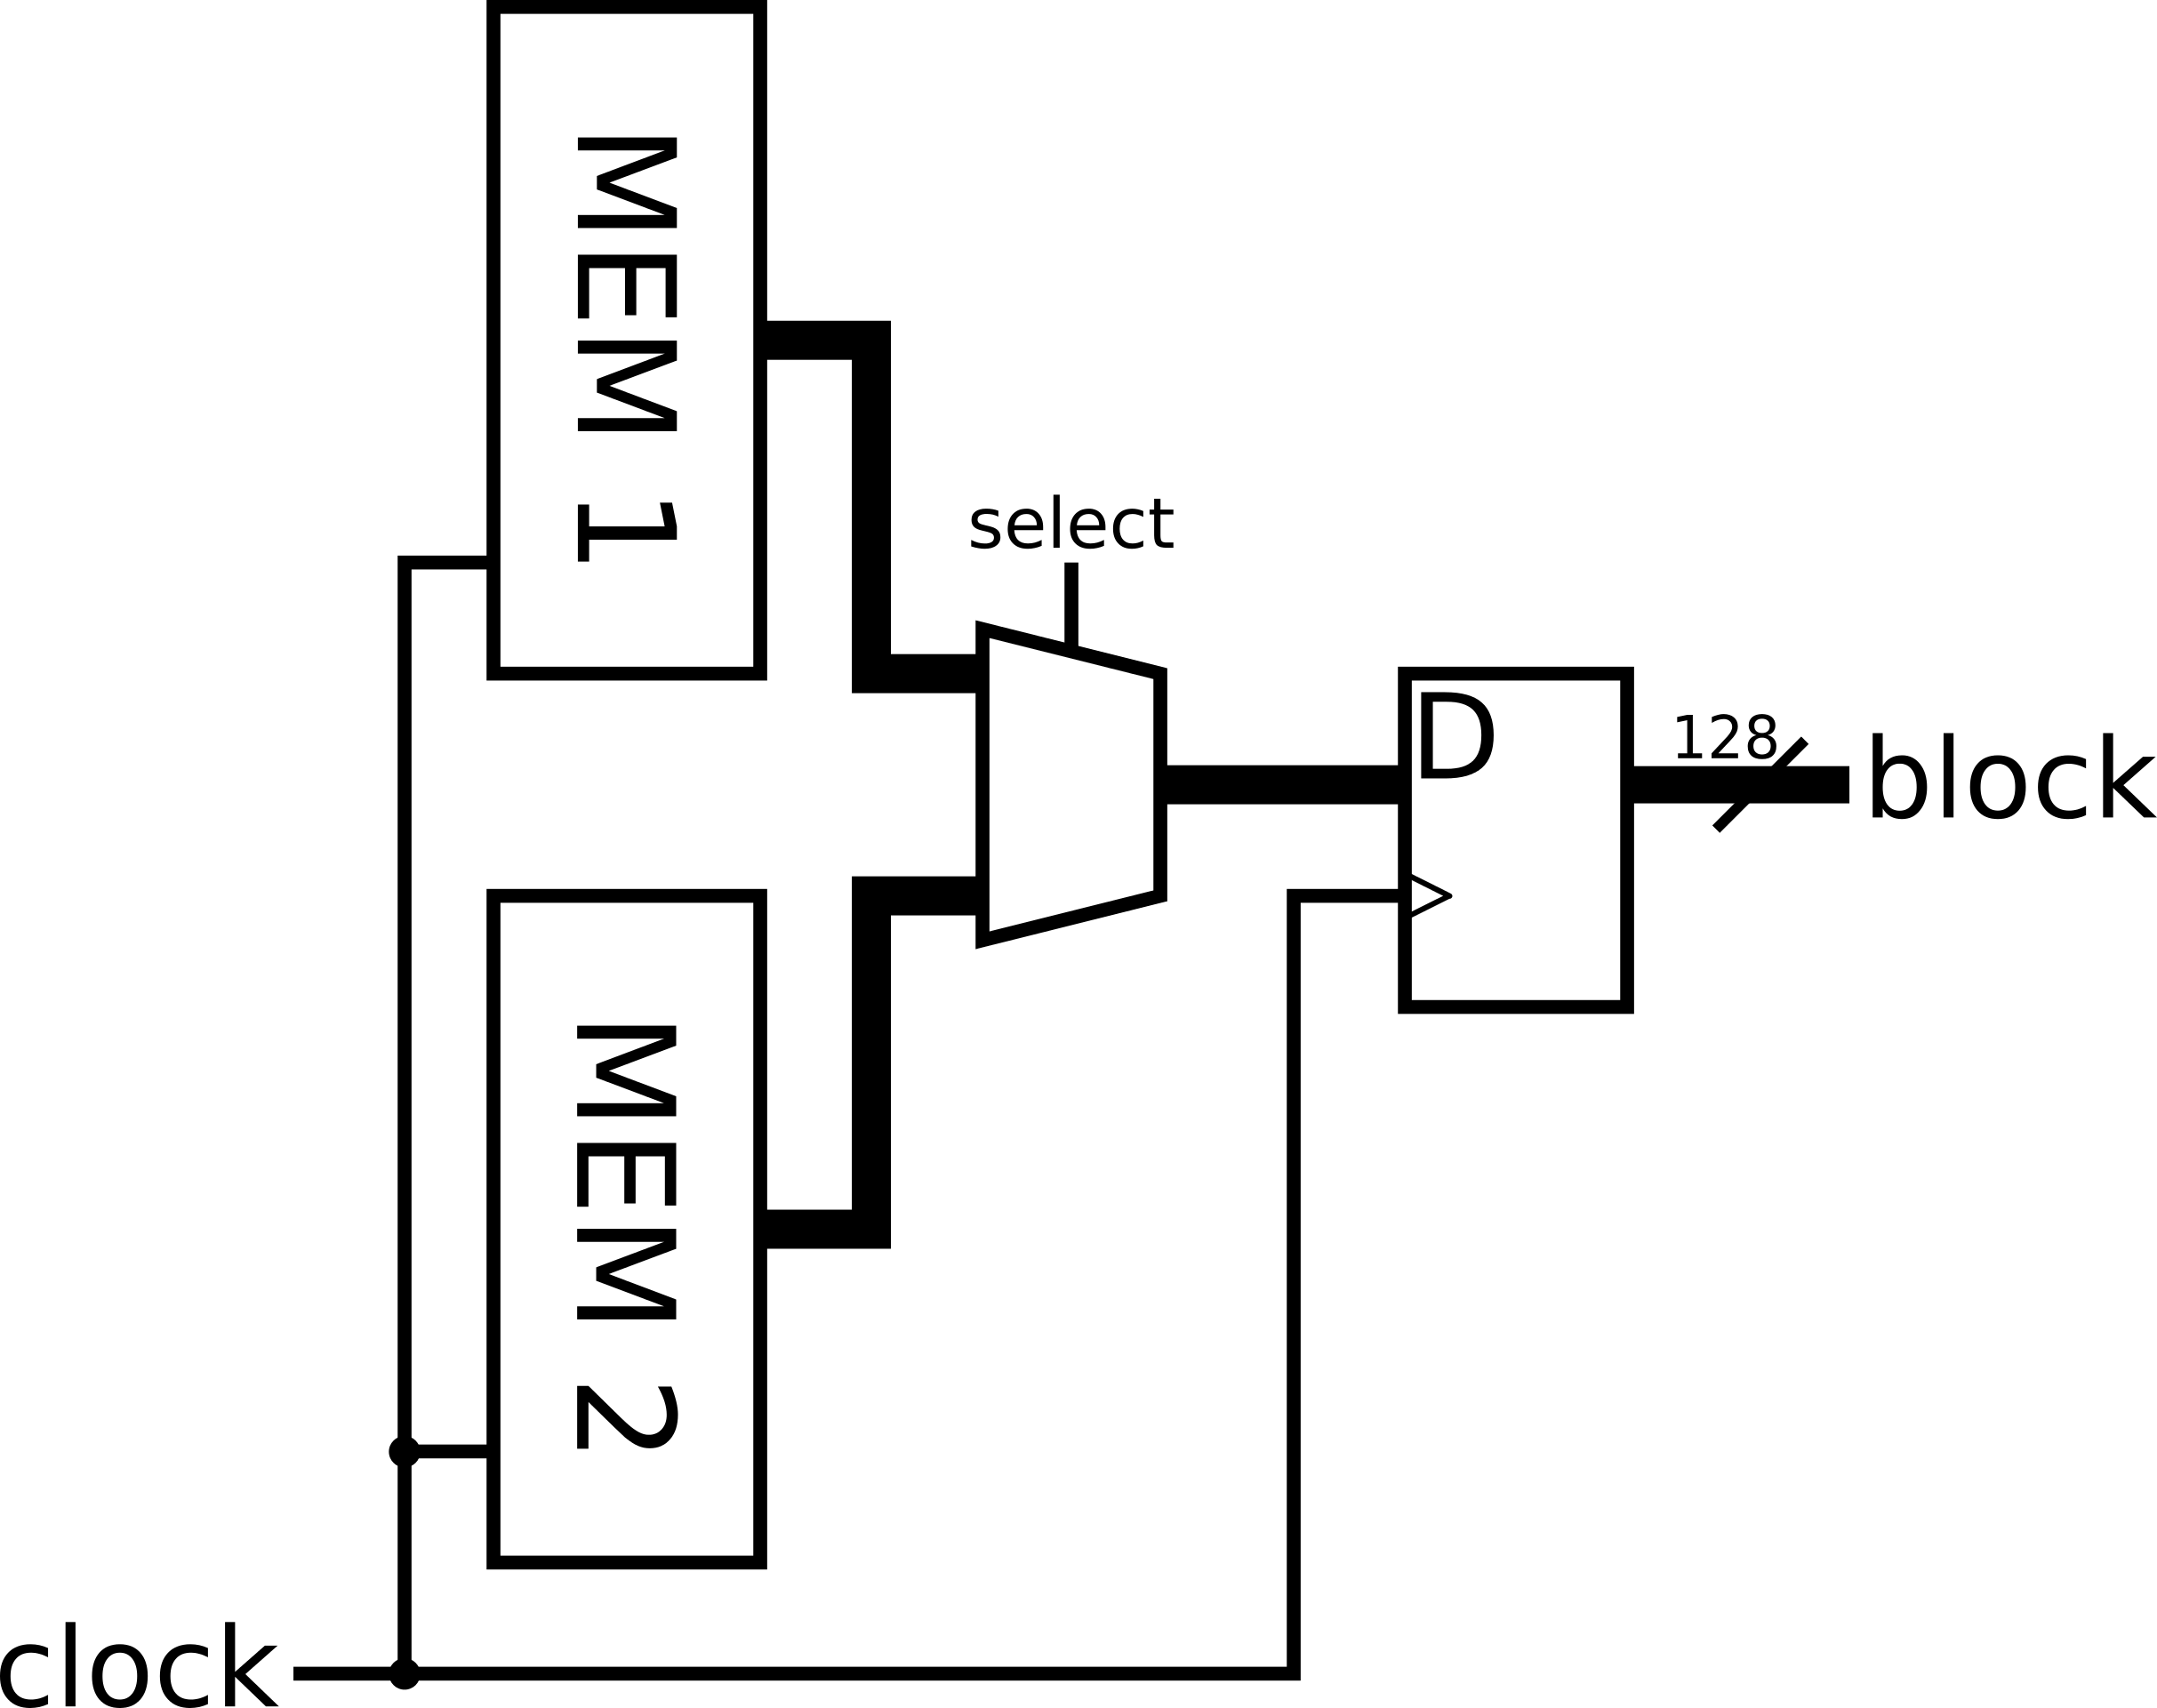
\includegraphics[scale=3]{memory-arrangement}
\caption{Memory solution based on multiplexer}
\label{fig:memory-arrangement}
\end{figure}

Using more banks of ROM was tesed, but adding more resulted in decreased performance due to lack of enough routing resources in FPGA. This testing design was capable of operating at highest frequency and it was chosen to be used for making all frequency measurements.

\subsubsection{Queue based memory solution}
Second testing design (fig. \ref{fig:memory-queue}) that was considered is based on a looped queue of D flip-flops and uses only one bank of ROM - 128 bits wide, 32 blocks deep. Every 33 clock cycles a new block of data is fed to queue at position 0. This results in filling entire queue with test data after $32 * 32 + 1$ clock cycles. After this time stream of testing data is derived from output of one flip-flop in the queue. This approach results in ROM having to operate at only $\frac{1}{33}$ of main clock frequency. This design for delivering data blocks to test module allows for operation at 520MHz. 

\begin{figure}[!h]
\centering
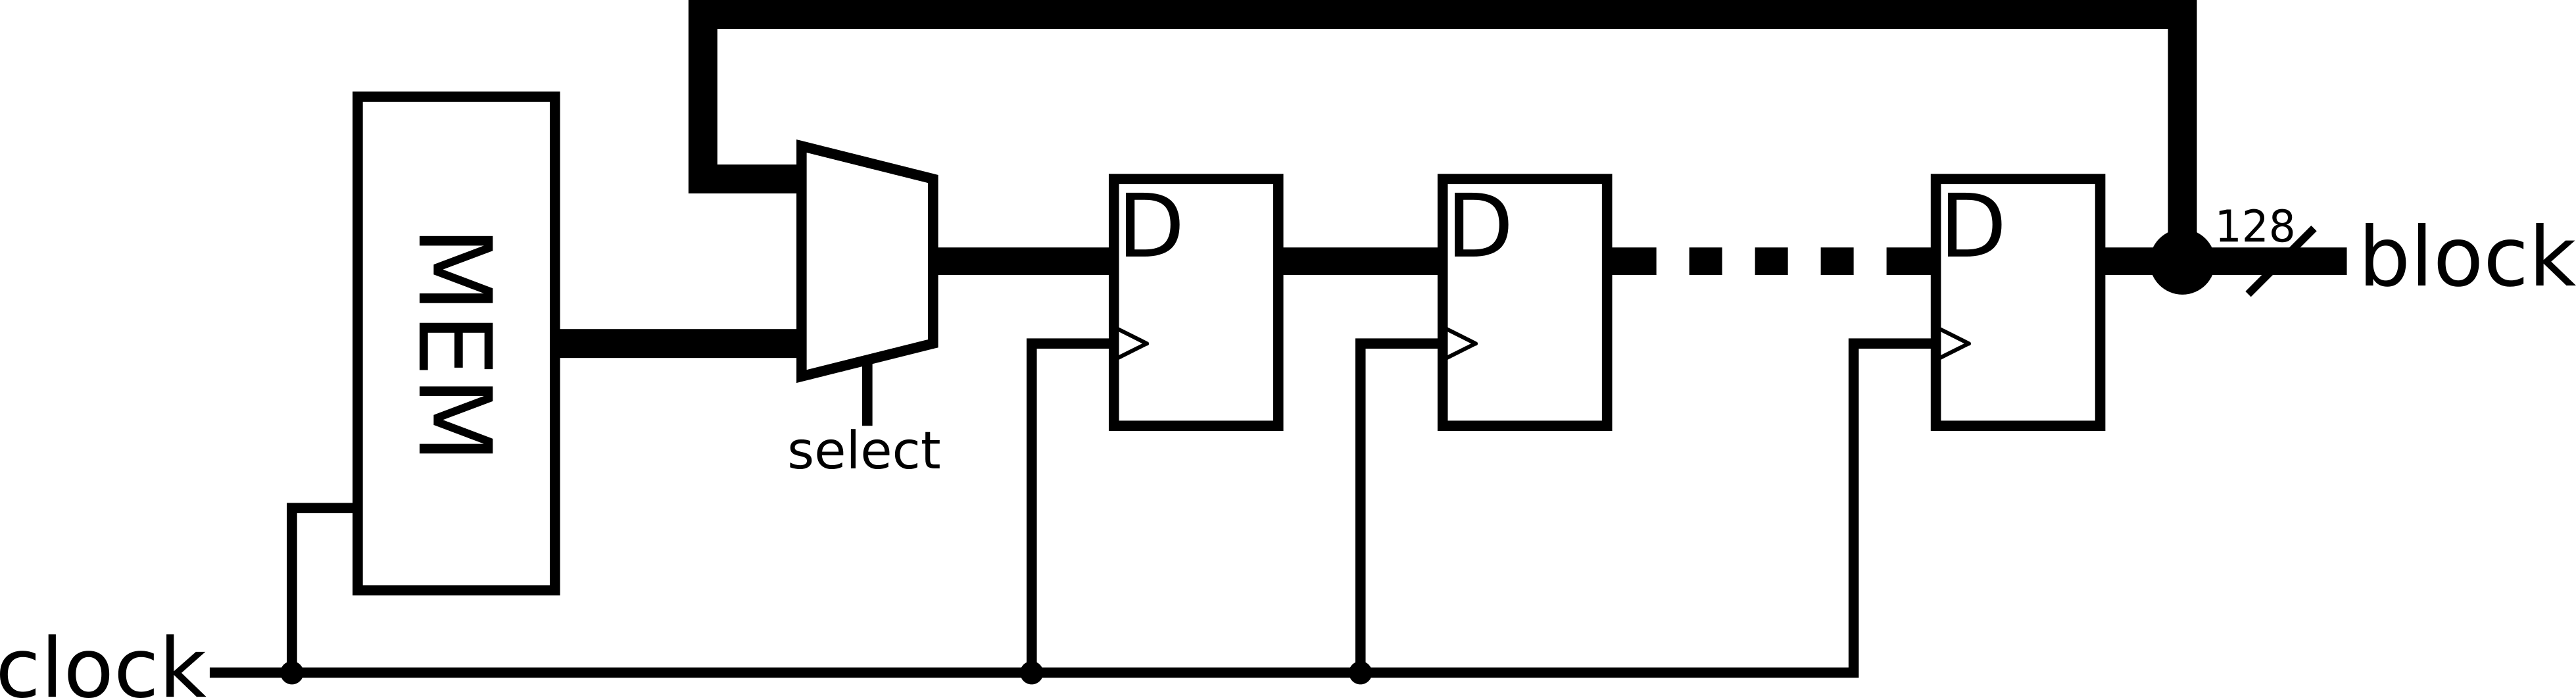
\includegraphics[scale=3]{memory-queue}
\caption{Memory solution based on queue}
\label{fig:memory-queue}
\end{figure}

Other similar designs with varying ROM depths and queue lenghts were tested, but they all performed similarly, and none of them were faster than multiplexer approach.


\subsubsection{Testing circuit}
Testing circuit (fig. \ref{fig:test-circuit}) provides blocks of plaintext and encryption keys to tested design, and compares (using $xor$ gates) calculated cyphertext with expected result. If a bit difference occurs, then tested circuit is considered unstable at given frequency.

\begin{figure}[!h]
\centering
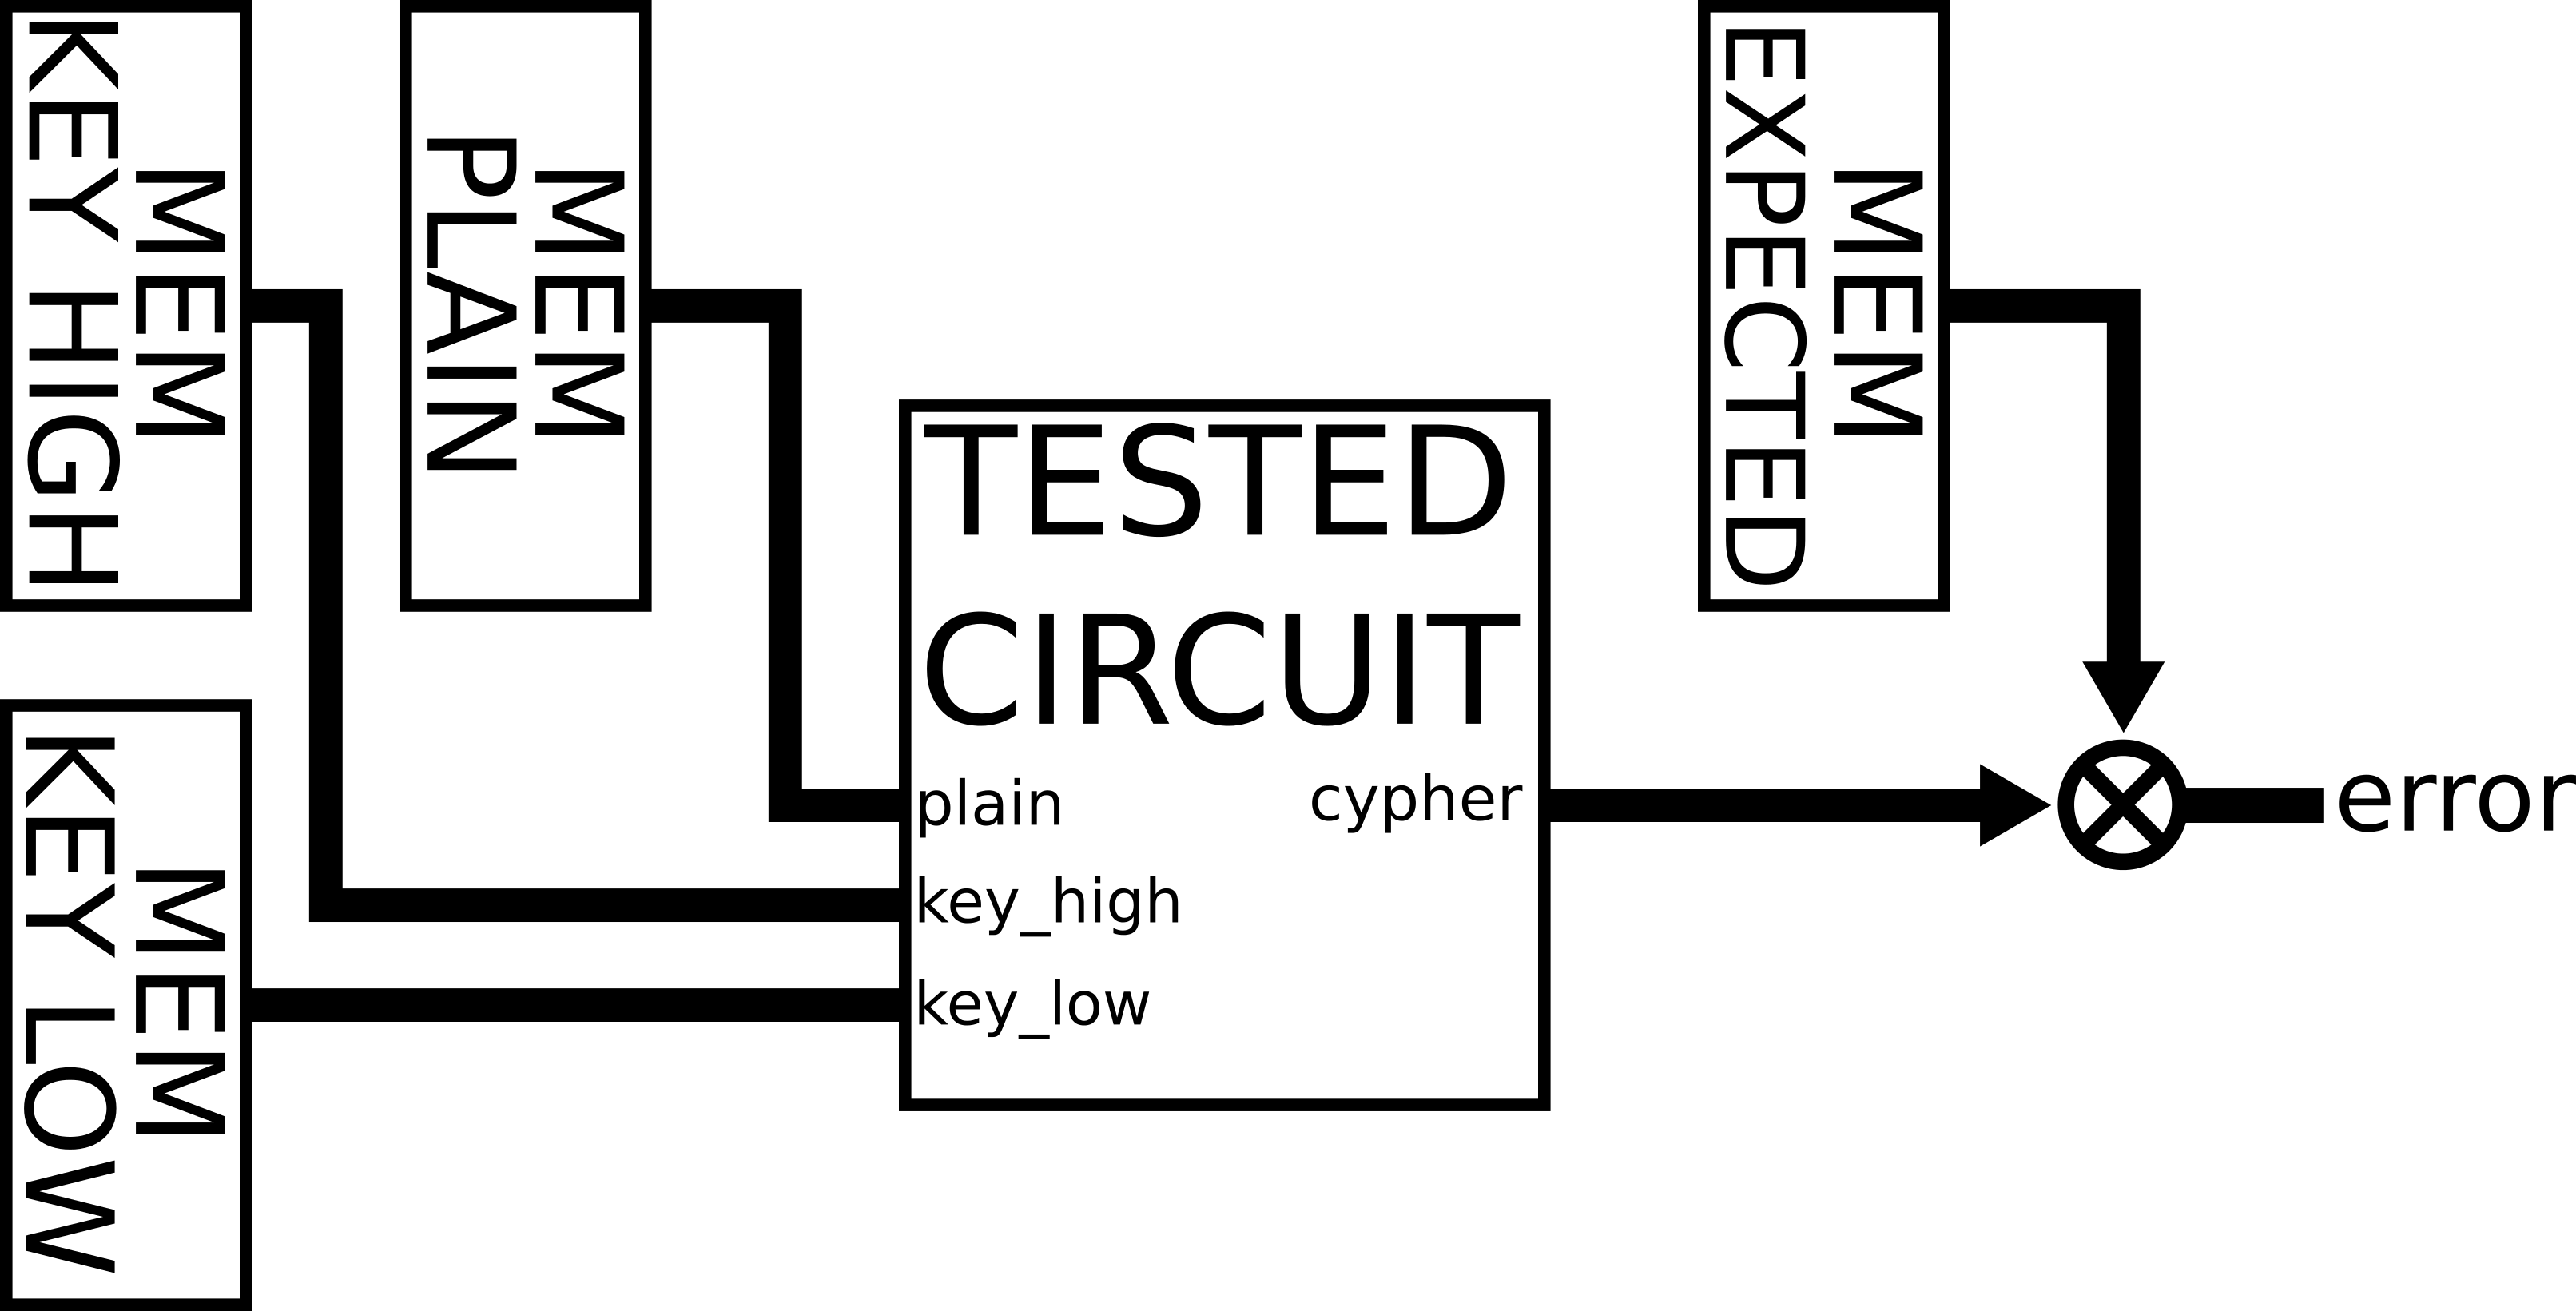
\includegraphics[scale=3]{test-circuit}
\caption{Testing circuit}
\label{fig:test-circuit}
\end{figure}

Data in expected result memory is initiated with an offset taking into account the number of pipeline stages in tested design.

This testing circuits consumes 806 ALM FPGA resources and 32768 on-chip memory bits.



\subsection{Logic utilization}
Logic utilization for each design was calculated based on compiler output - after each compilation Quartus software calculates how many FPGA logic elements the design uses. For each tested design number of logic elements in testing circuit (806) was subtracted to determine how much logic the actual AES encryption module utilizes.



\subsection{Correctness}
Correctness of the design was tested in two ways:
\begin{description}
\item[Wave form simulations] were used for simulating and testing sections of the design. This kind of testing was performed during development process.
\item[Testing of designs deployed in FPGA] was always performed along with performance testing (fig. \ref{fig:test-circuit}). Those tests were performed only after implementation of given part of circuit was completed and wave form simulation testing showed no issues.
\end{description}

Input data and expected results for testing of transformations, key expansion and entire encryption algorithm were taken from examples in AES encryption standard \cite{aes-standard}. For testing of smaller portions of the design input data was randomly generated and expected results were precalculated either maually or by implementing a utility script in python.

\section{Throughput optimized architecture}
\label{sec:throughput-optimized-architecture}

Throughput of AES encryption module is optimized by utilizing pipelining. To use this technique the design needs to be split into stages. To maximize benefits that pipelining brings signal propagation time through all stages needs to be roughly the same. Authors of \cite{vlsi} partitioned their design based on critical path length. My testing shows that this approach is suboptimal, and higher frequencies can be achieved by partitioning the design in a way that combinatorial logic for each output bit of a stage has no more than 4 inputs. This is due to how FPGA technology works and will be explained in more detail this section.

% \begin{table}[!h]
    % \label{table:sub-bytes-crit-path}
	% \centering
	% \begin{tabular}{| l | l |}
	% \hline
    % \textbf{Operation} & \textbf{Critical path} \\ \hline
% 
    % Multiplication by constant $\phi$ in $GF(2^2)$ & 1 XOR \\ \hline
% 
    % Multiplication by constant $\lambda$ in $GF(2^4)$ & 2 XOR \\ \hline
% 
    % Multiplication in $GF(2^2)$ & 2 XOR + 1 AND \\ \hline
% 
    % Multiplication in $GF(2^4)$ & 4 XOR + 1 AND \\ \hline
% 
    % Squaring in $GF(2^4)$ & 2 XOR \\ \hline
% 
    % Multiplicative inversion in $GF(2^4)$ & 3 XOR + 2 AND \\ \hline
% 
    % Mapping from $GF(2^8)$ to $GF((2^4)^2)$ & 4 XOR \\ \hline
% 
    % Mapping from $GF((2^4)^2)$ to $GF(2^8)$ + AES affine transformation & 4 XOR \\ \hline
% 
    % \end{tabular}
    % \caption{Critical path lengths for operations in SubBytes transformation}
% \end{table}
% 
% \begin{table}[!h]
	% \centering
	% \begin{tabular}{| l | l |}
	% \hline
    % \textbf{Transformation} & \textbf{Critical path} \\ \hline
	% MixColumns & 3 XOR \\ \hline
	% AddRoundKey & 1 XOR \\ \hline
	% ShiftRows & 0 \\ \hline
    % \end{tabular}
    % \caption{Critical path lengths for MixColumns, ShiftRows and AddRoundKey transformations}
% \end{table}
% 

\subsection{Low level FPGA chip analysis}
\label{sec:low-level-fpga}
To optimize a circuit for high frequency operation it is necessary to understand how FPGA technology works on low level. FPGA chips' archirectures may slightly vary, here we will focus on architecture of the chip that I used for testing - Altera Cyclone V \cite[Chapter 1]{altera-vol1}. For simplicity only elements relevant to this design will be covered here, detailed documentation is available in Cyclone V Handbook \cite{altera-vol1}.

FPGA chips consist of LABs (Logic Array Blocks), each of which contains 10 ALMs (Adaptive Logic Modules). ALMs are elements that make it possible to place arbitrary circuits in FPGA - they can be programmed to implement combinatorial logic functions, arithmetic functions, and registers.

Combinatorial logic is implemented in ALMS using LUTs (LookUp Tables) which contain high speed ROM memory. This memory is programmed with precomputed outputs for every possible combination of logic levels of input signals. LUTs take combinatorial logic inputs and use them as addresses to corresponding memory bits. Output of LUT is a bit read from memory which corresponds to provided inputs. An important consequence of this design feature is that for a LUT with N inputs it is irrelevant how complex the logic to be implemented is - as long as it has no more than N inputs it will always perform the same. This is because all outputs are precomputed and all it takes to determine the output is to read it from memory. If desired combinatorial logic has more than N inputs multiple LUTs will be required.

In Cyclone V chips each ALM contains two LUTs and four registers (D flip-flops). The registers, however, are wired in such a way that only two are relevant for this design - other two could be utilised if ALMs were used to implement arithmetic logic, which does not happen in AES encryption. LUTs in Cyclone V ALMs are capable of implementing different combinations of combinatorial logic, for this design the relevant combinations are:
\begin{itemize}
\item one 6-input LUT per ALM - uses up to 1 register, leaves at least one register unused
\item two 4-input LUTs per ALM - uses up to 2 registers
\end{itemize}
Combinatorial logic outputs can either be registered in the ALM they were calculated in or routed to another ALM without registering. For fastest operation in most cases it is desired to register them in the same ALM, because routing inside ALM is a lot faster than between ALMs. Routing outputs without registering is necessary when combinatorial logic has more inputs than a single ALM supports, or to move the register closer to other parts of the design to balance routing delays between different parts of the design.

% Conducted tests showed that for AES encryption maximum frequency was higher for designs using only 4-input LUTs. Analysis of compilation reports showed that using 6-input LUTs resulted in overall increased number or resources used, which resulted in longer routing paths between parts of the design, which ultimately slowed it down. This makes sence, because for 4-input LUTs ALMs are used more efficiently - more combinatorial logic could be implemented, and both registers could be used. The leftover register when using 6-input operation mode was observed not to be used often, because other signals were typically registered in same ALMs they were calculated in.
Conducted tests showed that for AES encryption maximum frequency was higher for designs using only 4-input LUTs. Analysis of compilation reports showed that using 6-input LUTs resulted in paths with longer signal propagarion time, which slowed the design it down. This makes sence, because for 4-input LUTs ALMs are used more efficiently - more combinatorial logic could be implemented, and both registers could be used. The leftover register when using 6-input operation mode was observed not to be used often, because other signals were typically registered in same ALMs they were calculated in.

Another important aspect of working with FPGA is that \textit{Place and Route} compilation phase, which is responsible of finding optimal placement of the design in FPGA chip, tackles an NP-hard problem. This phase therefore uses heuristics to produce an approximation of best possible solution. It is possible that final placement of the design will be different for each compilation attempt. This behaviour was observed during testing, but maximum frequency for given design remained stable between compilation attempts. The longest routes for each compilation were different every time, but leading trends were similar (eg. most routes from top 10 failing ones were between pipelined stages X and Y).



\subsection{Analysis of pipelied stages of equal critical path lengths}
As an entry point for my research I implemented the circuit proposed in \cite[Fig. 11]{vlsi} (for r=7 pipeline stages). Testing of this design showed that all transformations individualy could run at frequencies exceeding 500MHz (close to or at testing circuits max frequency of 530MHz). One full round could run at this frequency as well, but adding more consecutive rouds resulted in decrease of frequency due to FPGA resource congestion resulting in longer routing paths. Full AES encryption circuit, which consists of 15 rounds, was capable of operating at \textbf{375MHz} and consumes 15123 ALM resources.

Analysis of paths with longest propagation time presented in compilation report showed that typically they consisted of two or more ALMs used for calculating combinatorial logic. This was due to the fact that this design used pipelining stages which for calculating each output bit required more than 6 inputs. This forced utilising multiple ALMs between registers, which resulted in long routing delays.

The conclusions of this research were:
\begin{itemize}
\item To achieve higher frequency it was necessary to split the design into shorter pipelining stages.
\item Critical path length calculated as number of layers of logical gates is irrelevant (sec. \ref{sec:low-level-fpga}).
\item What is relevant is the number of input signals required for calculating each bit of stage output, which should be no higher than 6.
\item Routing delays are a significant factor contributing to maximum achievable frequency.
\item Reducing number of LUTs between registers is critical for high performance.
\end{itemize}

% Analysis of compilation reports showed that paths with longest signal propagation time, which were responsible for limiting maximum achievable frequency, 



% SubBytes transformation is by far the most complex one and it should be split into multiple pipelined stages. MixColumns and AddRoundKey have short critical paths (3 and 1 respectively) and can be combined into a single stage with critical path of 4. ShiftRows only rearranges order of bits in AES state without using any logic gates, so it can be joined with other operations to form a stage.

% Performance testing indicated that stages with critical paths of 6 gates would be short enough to be able to operate at over 500MHz, which is enough to fully utilize used testing framework. It is also convenient, as such stage length makes it possible to use all operations (\ref{table:sub-bytes-crit-path}) without splitting them. It is worth noting, that given an FPGA chip capable of operating at higher frequencies, pipelining stages could be made shorter than what is considered here (critical path of 6).

% Each AES round is split into 6 pipeline stages as shown in fig. \ref{fig:round-split}.


\subsection{Design of optimal pipelining stages}
\label{sec:pipeline-stages-design}

First approach to optimization was to split pipelining stages so that thay used 4-input as well as 6-input LUTs. This approach resulted in increased performance, but analysis of compilation reports showed that paths with longest signal propagation time typically led through ALMs utilising 6-input operation mode. The circuit was therefore further redesigned to take advantage of only 4-input operation mode. Final design was capable of operating at \textbf{406MHz}, which is the highest achieved frequency for AES encryption observed in this research. The number of logic elements as reported by compiler for this design was \textbf{22411} (excluding 806 elements required for testing circuit).

This section will describe in detail how each operation in AES algorithm (sec. \ref{sec:aes-algorithm}) can be split into stages taking advantage of only 4-input LUT operation mode. To utilise this mode each registered output bit needs to depend on no more than 4 inputs.

% \paragraph{Top level design of SubBytes transformation}\mbox{}\\


\paragraph{Mapping $f(x)$ from $GF(2^8)$ to $GF((2^4)^2)$}\mbox{}\\
Output bits of this operation depend on as much as 7 input bits, therefore to make it use only 4-input LUTs it is necessary to split it into two substages (\ref{eg:f-split}) (fig. \ref{fig:f-split}) -- $f_a$ (\ref{eq:mul_delta_a}) and $f_b$ (\ref{eq:mul_delta_b}).

\begin{equation}
\label{eg:f-split}
f(x) = f_b \circ f_a(x)
\end{equation}

\begin{figure}[!h]
\centering
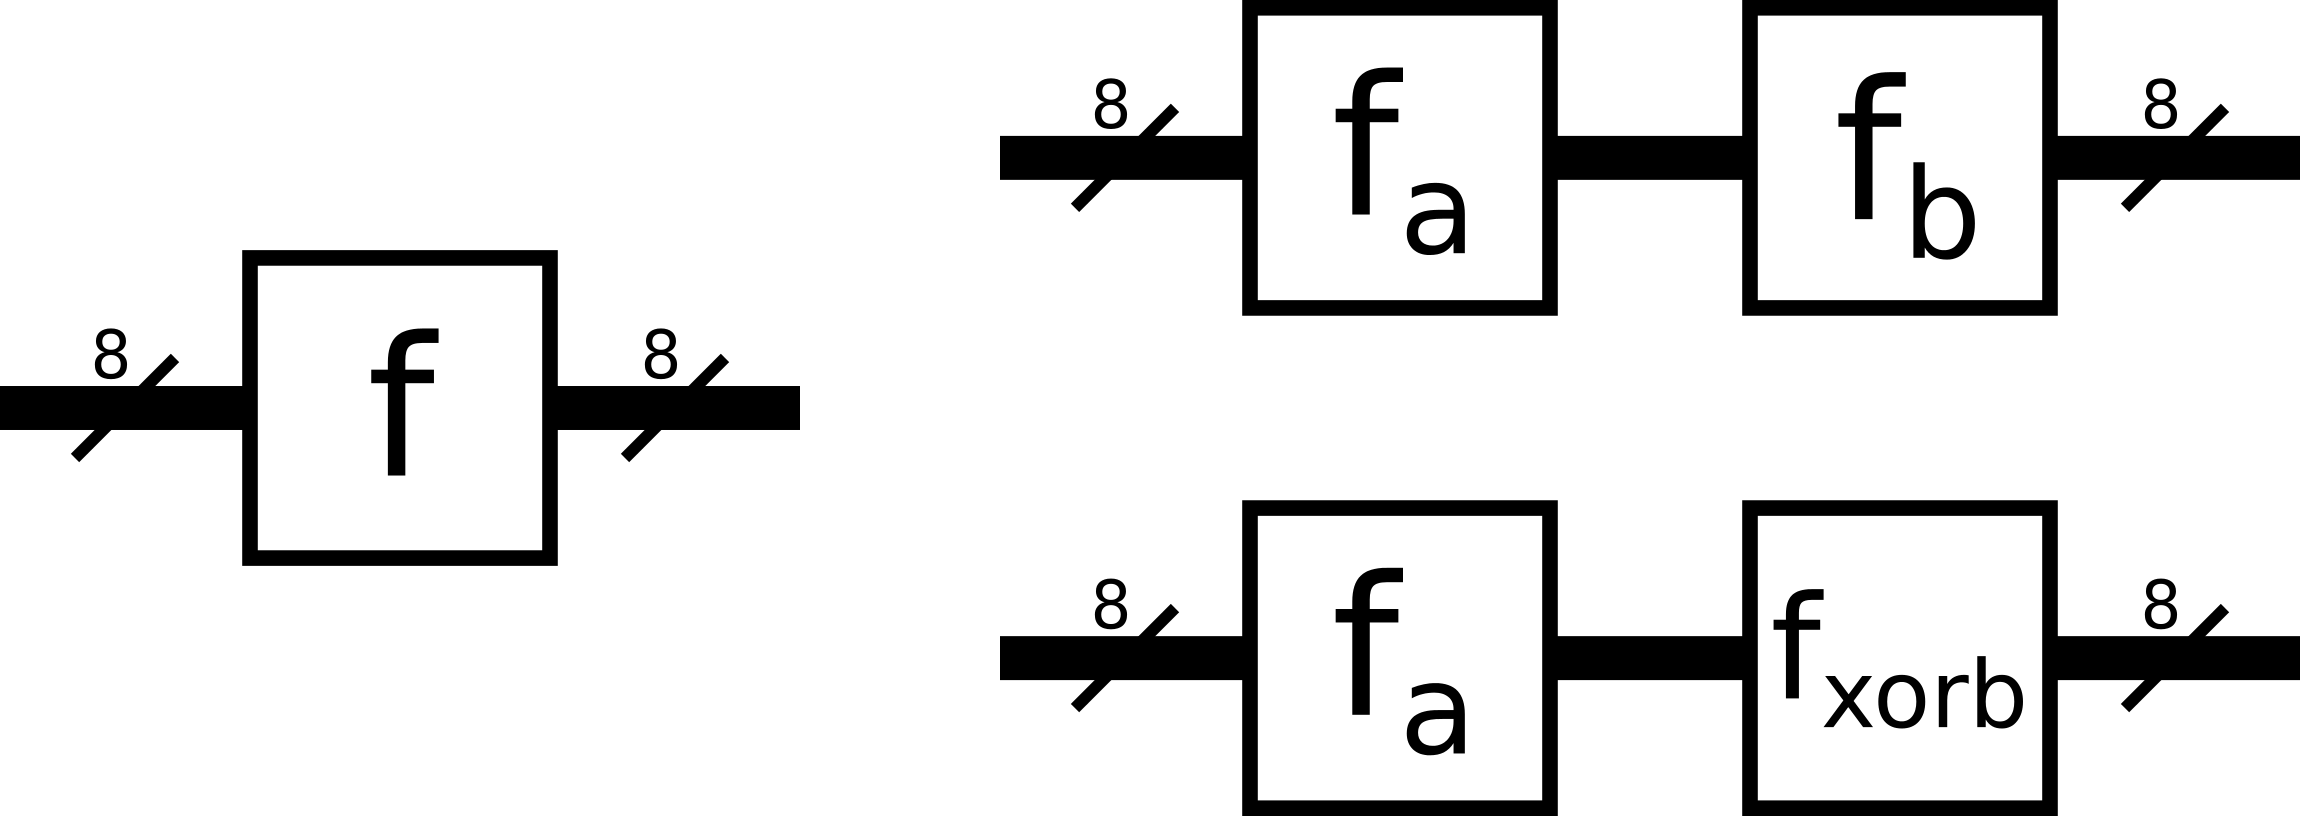
\includegraphics[scale=4]{f-split}
\caption{Decomposition of mapping $f(x)$ from $GF(2^8)$ to $GF((2^4)^2)$ into two stages}
\label{fig:f-split}
\end{figure}

\begin{equation}
\label{eq:mul_delta_a}
\begin{aligned}
b_{a0}    &= b_0                    \\
b_{a1}    &= b_1                    \\
b_{a2}    &= b_2                    \\
b_{a4}    &= b_4                    \\
b_{a5}    &= b_5                    \\
b_{a6}    &= b_6                    \\
b_{a7}    &= b_7                    \\
b_{a23}   &= b_2 + b_3              \\
b_{a567}  &= b_5 + b_6 + b_7        \\
b_{a1234} &= b_1 + b_2 + b_3 + b_4
\end{aligned}
\end{equation}

\begin{equation}
\label{eq:mul_delta_b}
\begin{aligned}
b'_0 &= b_{a0} + b_{a1} + b_{a6}           \\
b'_1 &= b_{a1} + b_{a4} + b_{a6}           \\
b'_2 &= b_{a7} + b_{a1234}                 \\
b'_3 &= b_{a1} + b_{a2} + b_{a6} + b_{a7}  \\
b'_4 &= b_{a1} + b_{a5} + b_{a7} + b_{a23} \\
b'_5 &= b_{a5} + b_{a7} + b_{a23}          \\
b'_6 &= b_{a6} + b_{a7} + b_{a1234}        \\
b'_7 &= b_{a5} + b_{a7}                    
\end{aligned}
\end{equation}

In SubBytes transformation after mapping $f(x)$ from $GF(2^8)$ to $GF((2^4)^2)$ high and low words of the result are xored together. This operation can be performed concurently with $f_b(x)$ mapping to avoid creating a separate stage only for a xor operation.

\begin{equation}
\begin{aligned}
f_{xor}(x) &= f(x)_{0123} + f(x)_{4567} \\
f_{xor}(x) &= f_{xorb} \circ f_a(x)
\end{aligned}
\end{equation}

\begin{equation}
\label{eq:mul_delta_xor}
\begin{aligned}
b_{xorb0} &= b_{a0} + b_{a23} + b_{a567}       \\
b_{xorb1} &= b_{a1234} + b_{567}               \\
b_{xorb2} &= b_{a6}                            \\
b_{xorb3} &= b_{a1} + b_{a2} + b_{a5} + b_{a6}
\end{aligned}
\end{equation}

From equations (\ref{eq:mul_delta_a}), (\ref{eq:mul_delta_b}) and (\ref{eq:mul_delta_xor}) it is apparent that each stage output bit depends on no more than 4 inputs.




\paragraph{Mapping $f^{-1}(x)$ from $GF((2^4)^2)$ to $GF(2^8)$ combined with AES affine transformation}\mbox{}\\
Analoguously to mapping $f(x)$ from $GF(2^8)$ to $GF((2^4)^2)$, mapping $f^{-1}(x)$ from $GF((2^4)^2)$ to $GF(2^8)$ combined with affine transformation (\ref{sec:comb-theory}) (\ref{eq:fa-split}) (fig. \ref{fig:fa-split}) should be split into two substages --  $f^{-1}_a$ (\ref{eq:mul_delta_inf_a}) and $f^{-1}_b$ (\ref{eq:mul_delta_inf_b}).

\begin{equation}
\label{eq:fa-split}
\begin{aligned}
f^{-1}(x) &= f_b^{-1}(x) \circ f_a^{-1}(x) \\
\end{aligned}
\end{equation}

\begin{figure}[!h]
\centering
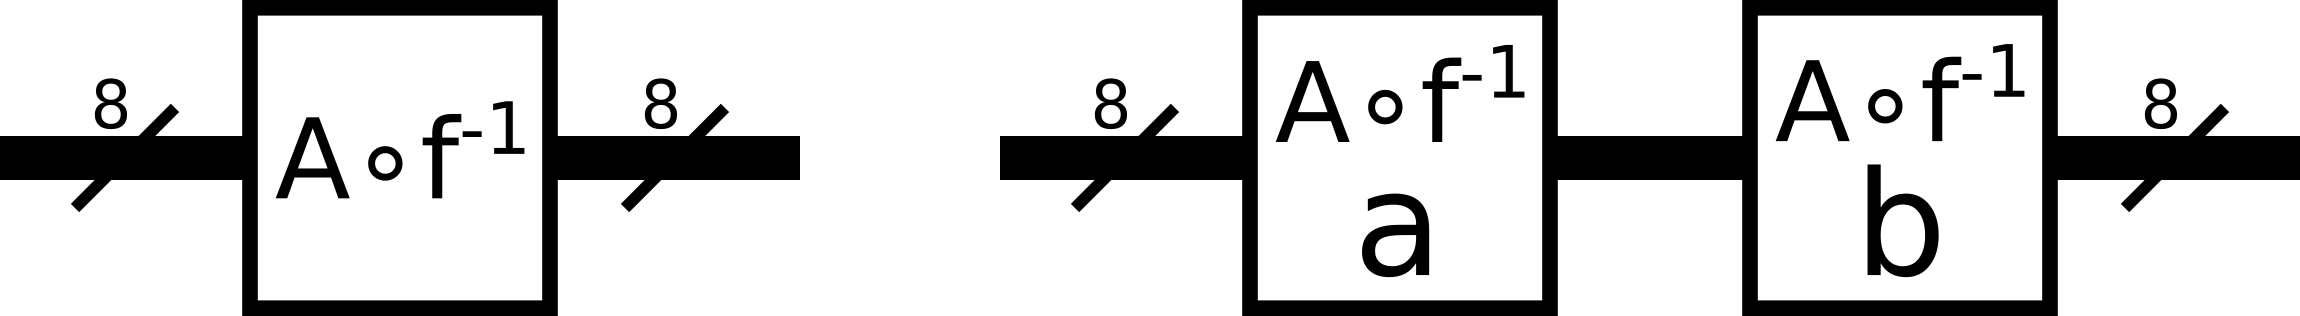
\includegraphics[scale=4]{fa-split}
\caption{Decomposition of mapping $f^{-1}(x)$ from $GF((2^4)^2)$ to $GF(2^8)$ combined with AES affine transformation into two stages}
\label{fig:fa-split}
\end{figure}


\begin{equation}
\label{eq:mul_delta_inf_a}
\begin{aligned}
b_{a0}    &= b_0                    \\
b_{a7}    &= b_7                    \\
b_{a23}   &= b_2 + b_3              \\
b_{a012}  &= b_0 + b_1 + b_2        \\
b_{a023}  &= b_0 + b_2 + b_3        \\
b_{a456}  &= b_4 + b_5 + b_6        \\
b_{a0147} &= b_0 + b_1 + b_4 + b_7  \\
b_{a27N}  &= b_2 + b_7 + 1          \\
b_{a67N}  &= b_6 + b_7 + 1            
\end{aligned}
\end{equation}

\begin{equation}
\label{eq:mul_delta_inf_b}
\begin{aligned}
b'_0 &= b_{a012} + b_{67N}           \\
b'_1 &= b_{a0} + b_{a7} + 1          \\
b'_2 &= b_{a023} + b_{a456}          \\
b'_3 &= b_{a012}                     \\
b'_4 &= b_{a0147}                    \\
b'_5 &= b_{a27N}                     \\
b'_6 &= b_{a456} + b_{a7} + 1        \\
b'_7 &= b_{a23} + b_{a7}                    
\end{aligned}
\end{equation}

From equations (\ref{eq:mul_delta_inf_a}) and (\ref{eq:mul_delta_inf_b}) it is apparent that each stage output bit depends on no more than 4 inputs. Note that $xor$ with $1$ value is merely a $not$ operation, and it does not increase input count. It is also true that all outputs of $f_b^{-1}(x)$ stage depend on no more than 2 inputs, so they can be xored with 2 other independent inputs to form a stage, which is important for a stage in key expansion pipeline.




\paragraph{Multiplicative inversion in $GF(2^4)$}\mbox{}\\
This operation has only 4 inputs, so it is can already be implemented using a 4-input LUT.

\paragraph{Multiplication by constant $\phi$ in $GF(2^2)$}\mbox{}\\
This operation has only 2 inputs, so it is can already be implemented using a 4-input LUT. 

\paragraph{Multiplication by constant $\lambda$ in $GF(2^4)$}\mbox{}\\
This operation has only 4 inputs, so it is can already be implemented using a 4-input LUT. Moreover, it is only used as part of SubBytes transformation directly after squaring in $GF(2^4)$. Because squaring takes only 4 inputs, and multiplication by $\lambda$ operates only on output of squaring, those two operations can be combined into single stage. Such merging only increases length of critical path of the stage (which is irrelevant) but does not increase number of inputs, which is still 4.


\paragraph{Multiplication in $GF(2^2)$}\mbox{}\\
This operation has only 4 inputs, so it is can already be implemented using a 4-input LUT. Every output depends on at most 3 inputs, so it is possible to xor each of them with a signal that does not depend on anything (was just registered).

\paragraph{Multiplication in $GF(2^4)$}\mbox{}\\
This operation has 8 inputs, so it is necessary to split it into two stages (fig. \ref{fig:mul-gf4-split}).

\begin{figure}[!h]
\centering
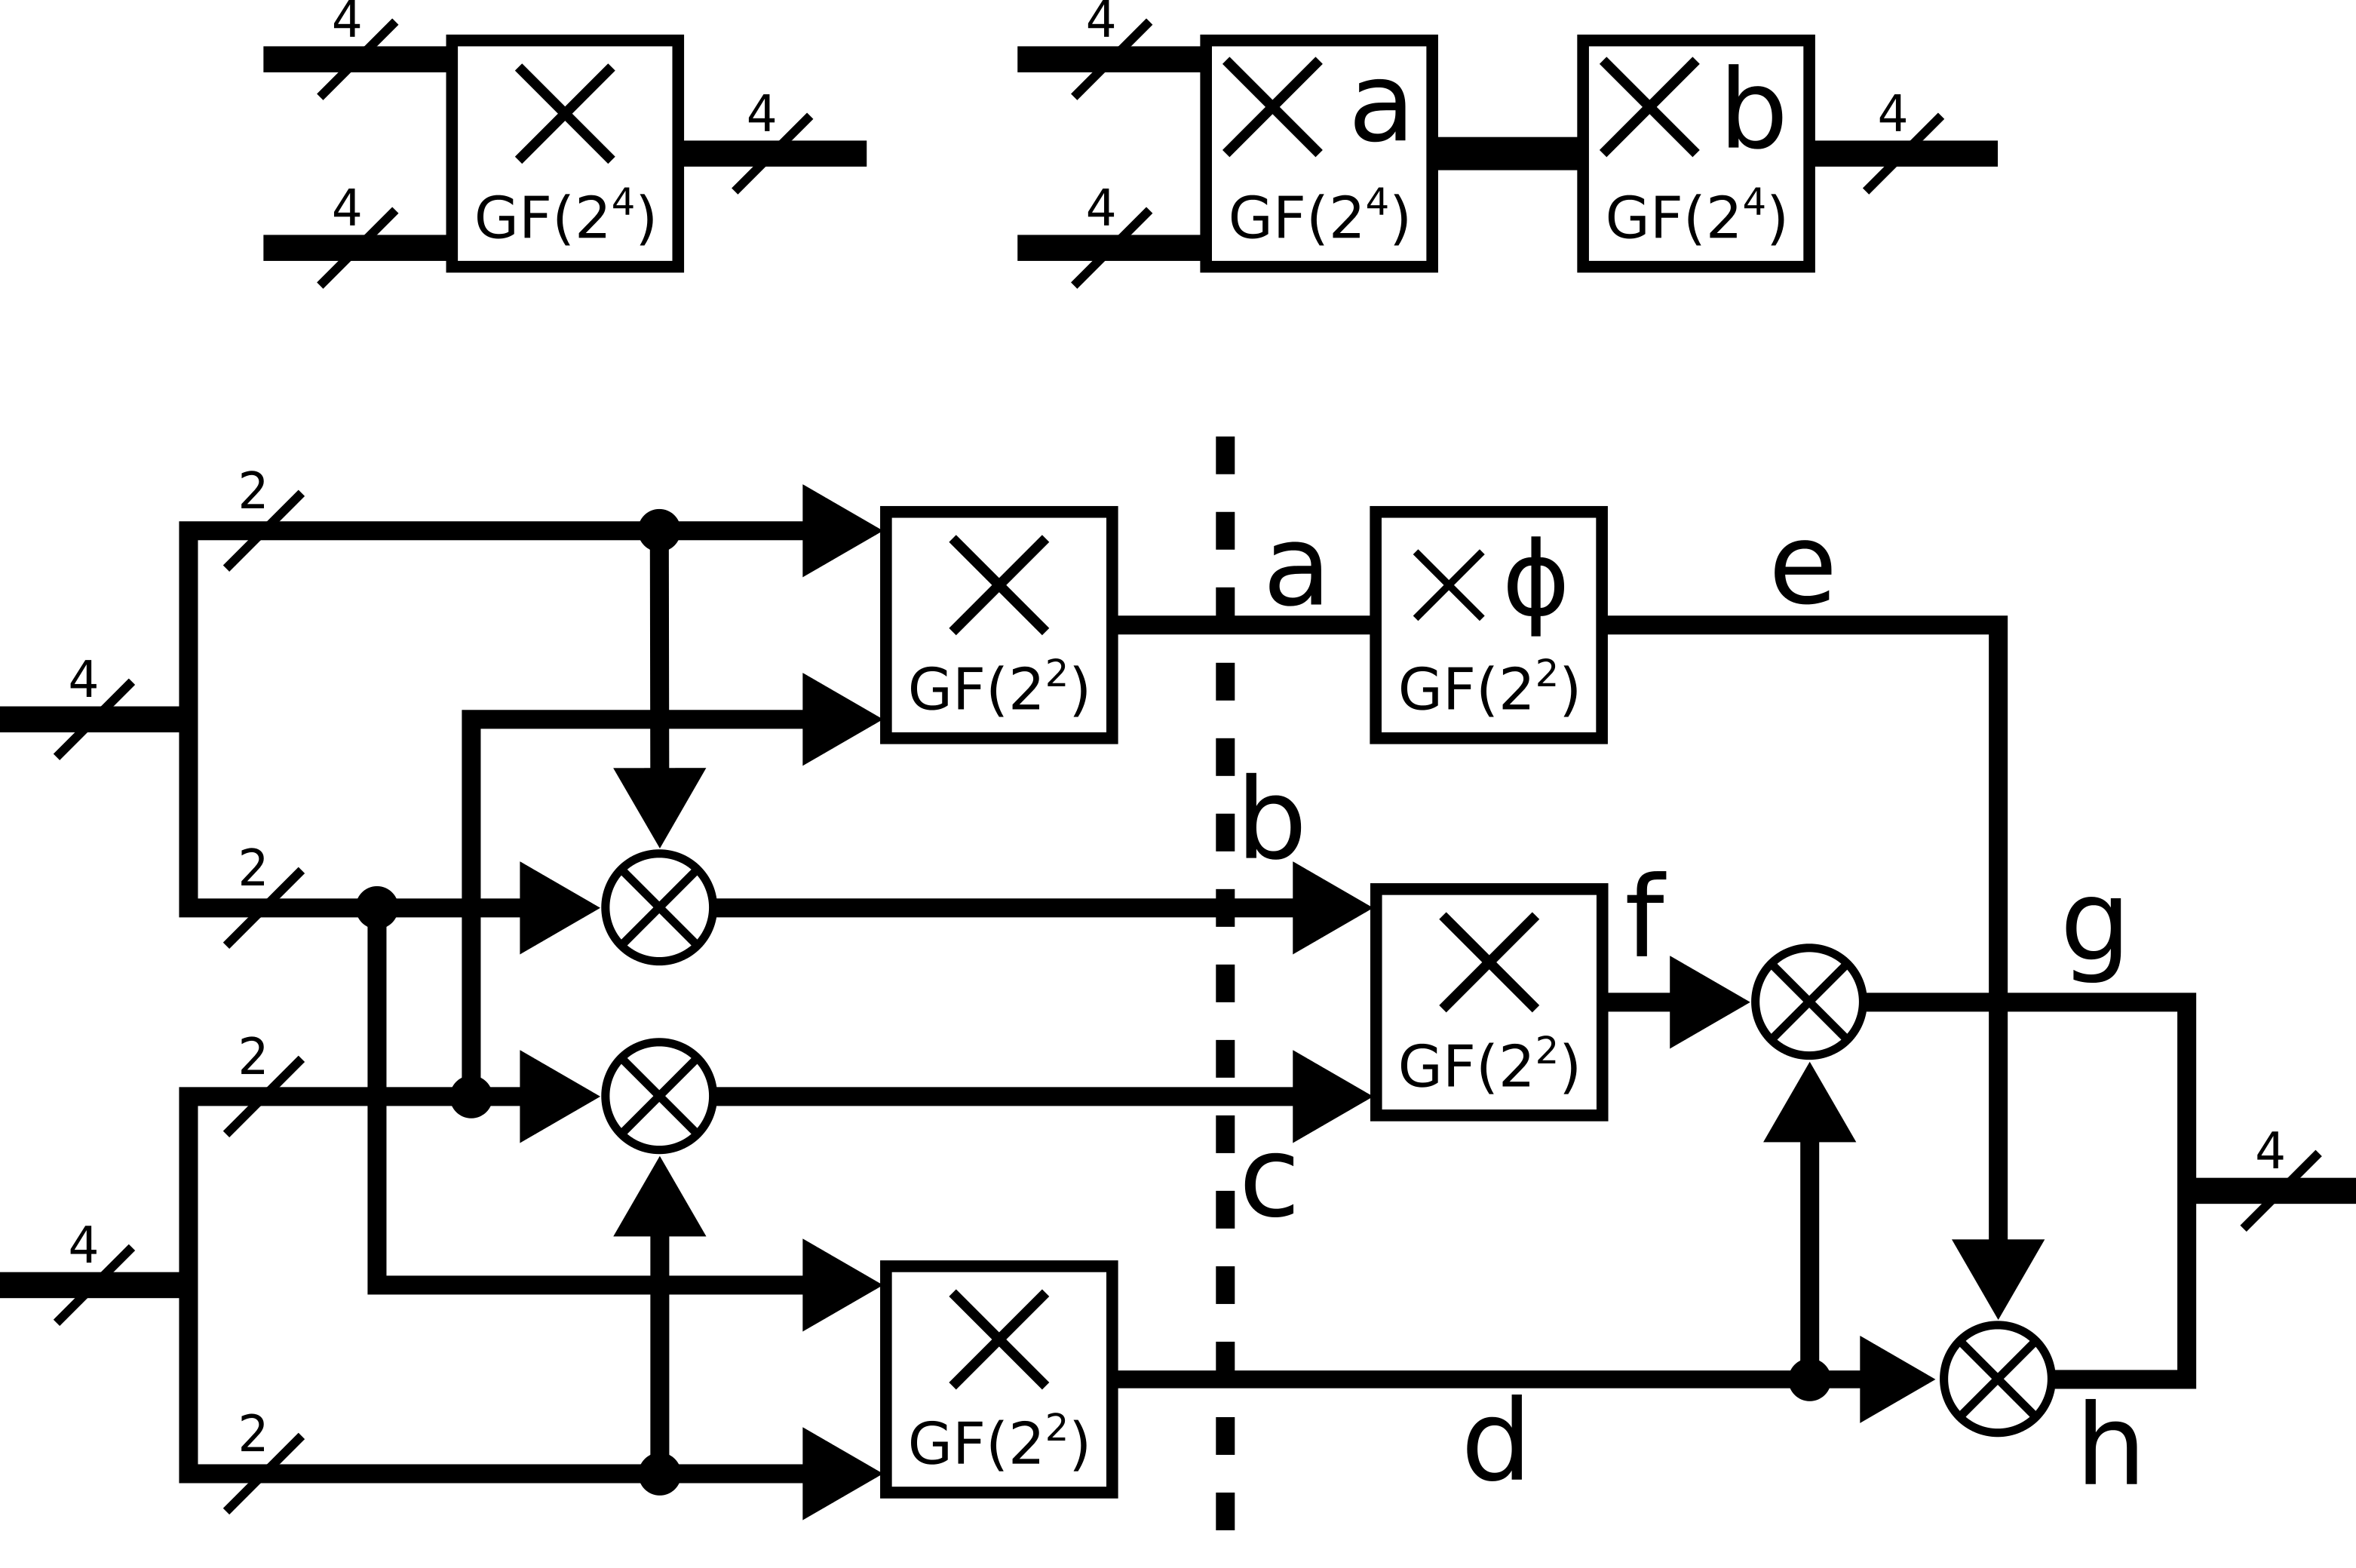
\includegraphics[scale=4]{mul-gf4-split}
\caption{Decomposition of multiplication in $GF(2^4)$ into two stages}
\label{fig:mul-gf4-split}
\end{figure}

This split uses only 4-input LUT operation mode, because:
\begin{itemize}[nolistsep]
\item Each bit of signals $a$ and $d$ depends on no more than 3 input signals, because on their paths there are only multiplications in $GF(2^2)$, which have this property. 
\item Each bit of signals $b$ and $c$ depends only on 2 input signals, because they are xors.
\item Each bit of signal $e$ depends on no more than 2 input signals, because this is a property of multiplication by $\phi$.
\item Each bit of signal $f$ depends on no more than 3 input signals, because this is a property of multiplications in $GF(2^2)$.
\item Each bit of signal $g$ depends on no more than 4 input signals, because signals from $f$ are xored with independent signals.
\item Each bit of signal $h$ depends on no more than 3 input signals, because signals from $e$ are xored with independent signals.
\end{itemize}


\paragraph{Squaring in $GF(2^4)$}\mbox{}\\
This operation has only 4 inputs, so it is can already be implemented using a 4-input LUT.


\paragraph{ShiftRows transformation}\mbox{}\\
This transformation does not do combinatorial logic and thus can be joined with any other operation to form a stage.


\paragraph{MixColumns transformation}\mbox{}\\
Lets first notice that some output bits of multiplication by $\{02\}_{16}$ depend on 2 input signals, all of which are already $xors$. This means that outputs of multiplication blocks already depend on $2 * 2 = 4$ signals. Those outputs are than xored again, which results in exceeding 4-input limit. MixColumns transformation, therefore, needs to be split into two stages. It can be done as shown in figure \ref{fig:mix-columns-split}.

\begin{figure}[!h]
\centering
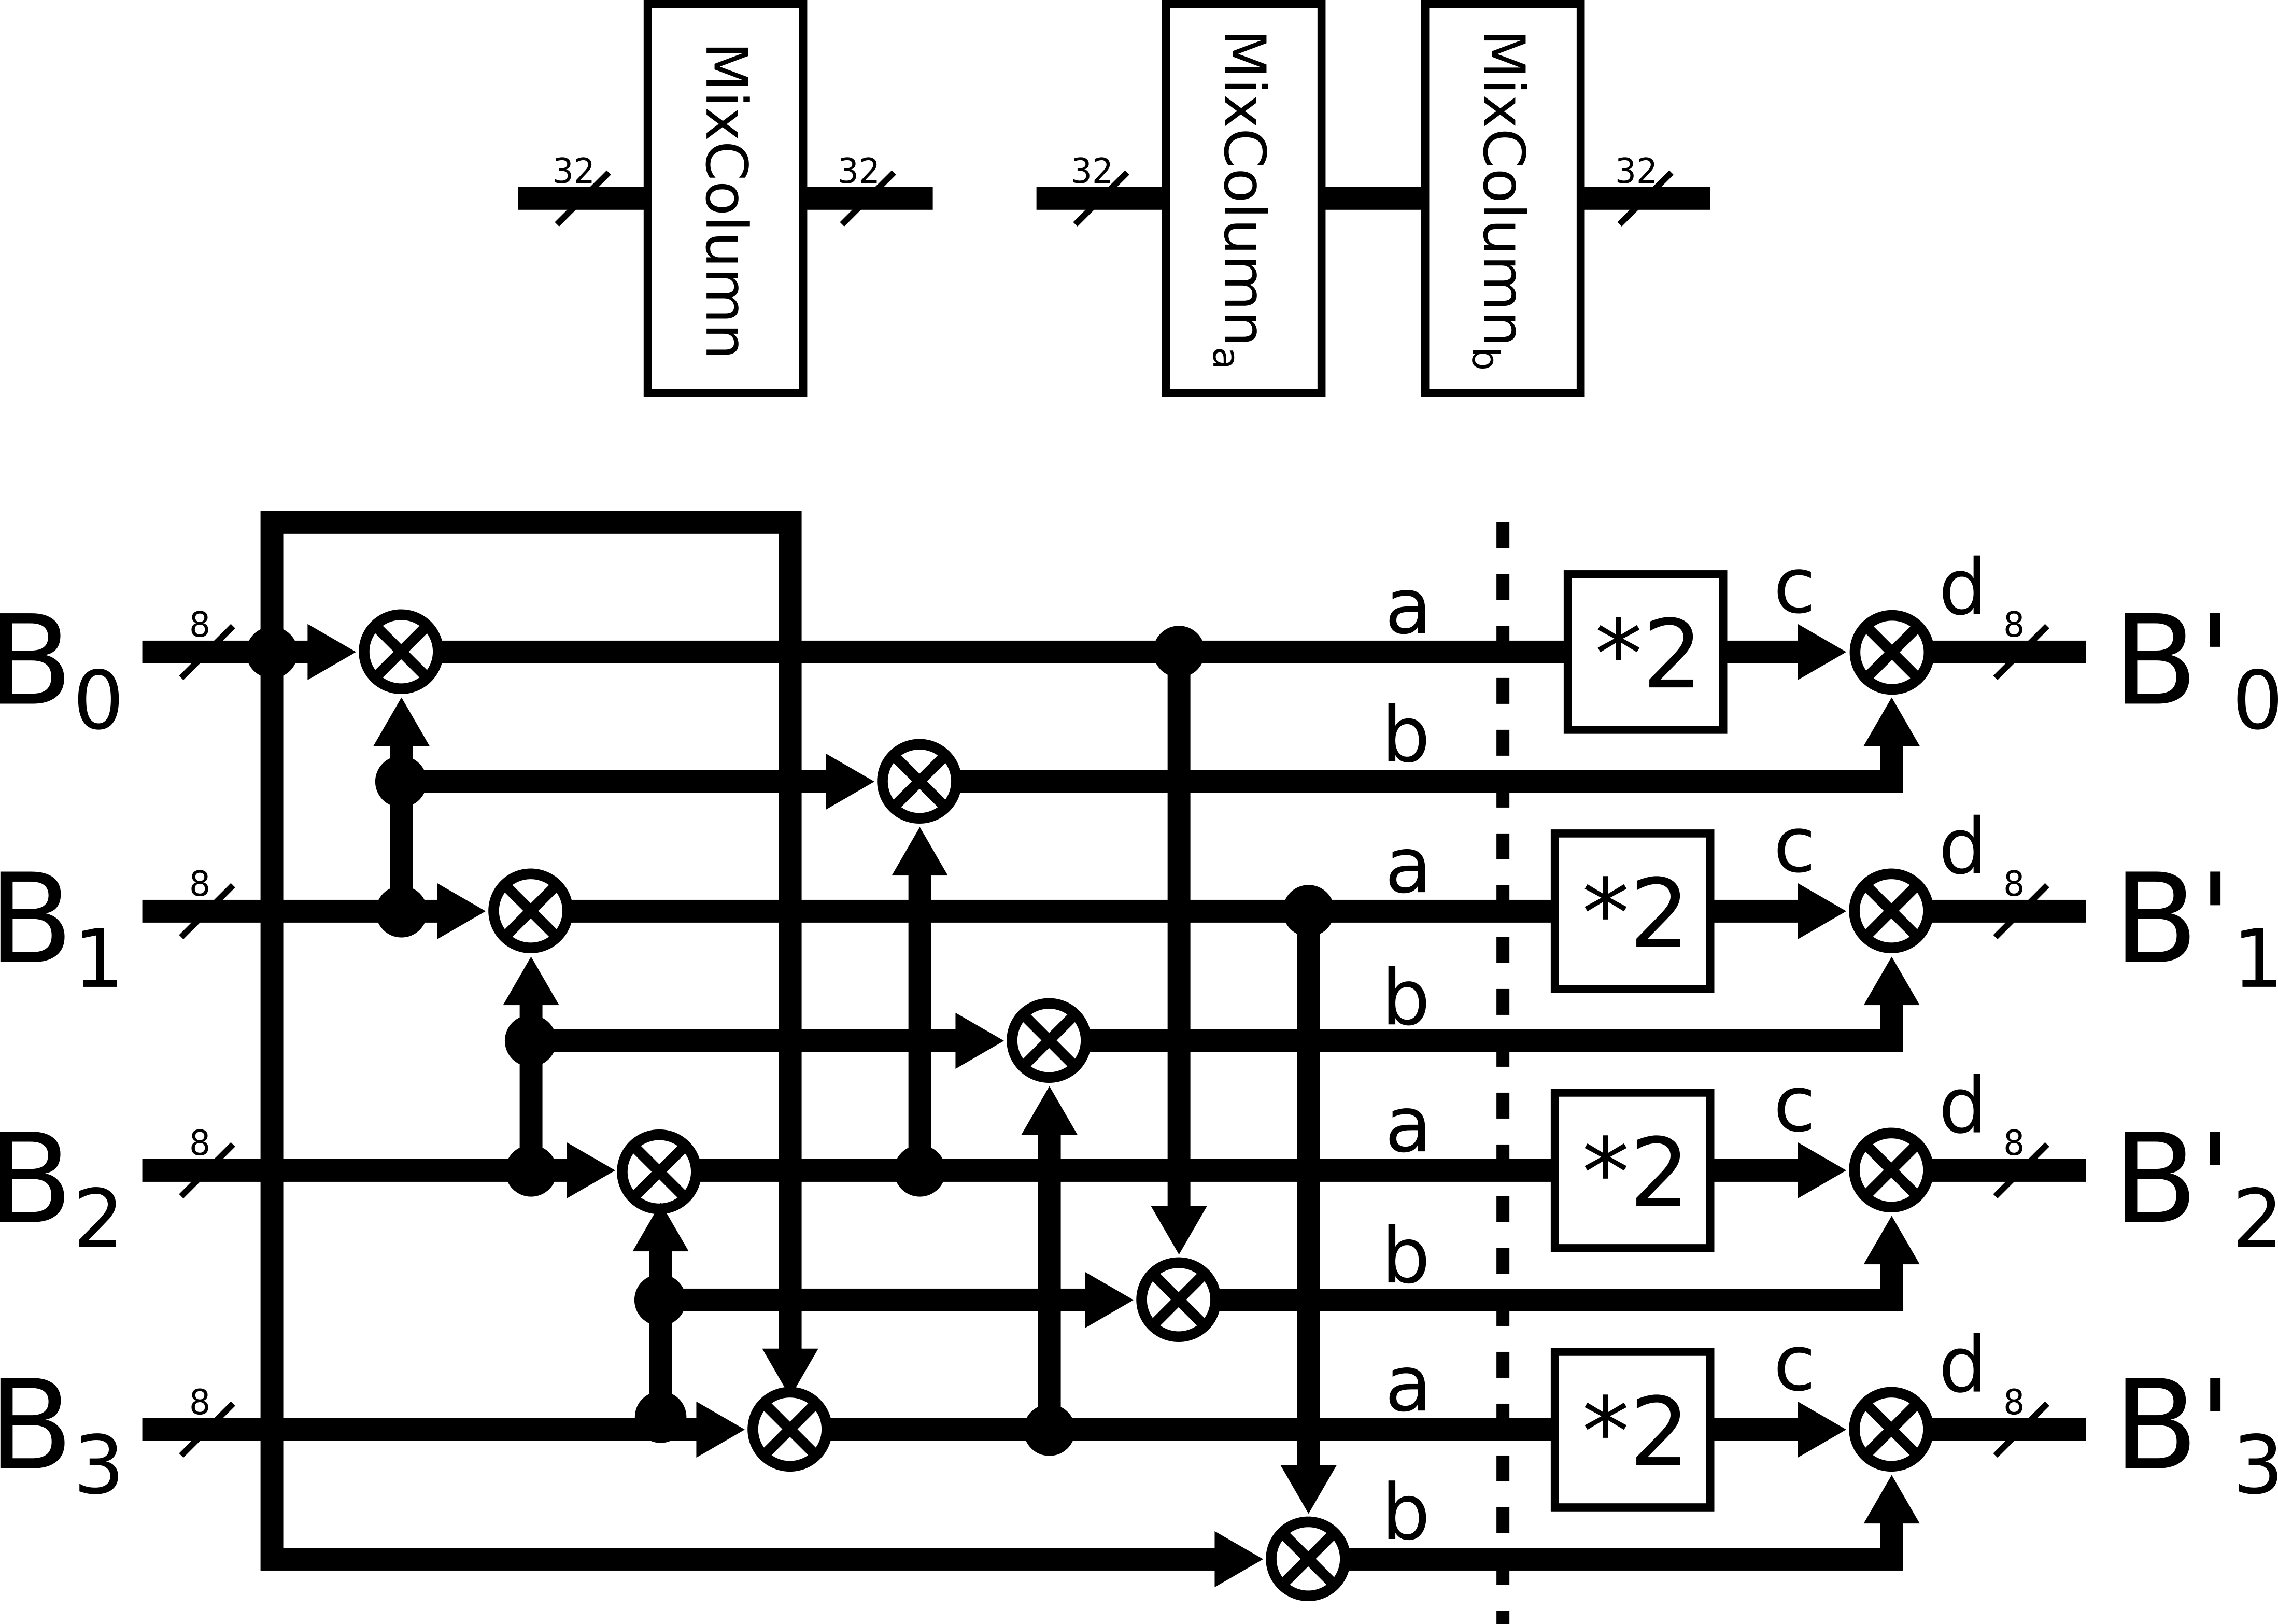
\includegraphics[scale=3]{mix-columns-split}
\caption{Decomposition of MixColumns transformation into two stages}
\label{fig:mix-columns-split}
\end{figure}

Those stages can be implemented using only 4-input LUTs, because:
\begin{itemize}[nolistsep]
\item Each bit of signals marked $a$ depends on 2 input signals.
\item Each bit of signals marked $b$ depends on 3 input signals.
\item Each bit of signals marked $c$ depends on no nore than 2 input signals.
\item Each bit of signals marked $d$ depends on no nore than 3 input signals.
\end{itemize}

Note that all output bits depend on no more than 3 input signals, which means that they can be xored with other independent inputs in one stage. This is useful for combining it with AddRoundKey transformation.


\paragraph{AddRoundKey transformation}\mbox{}\\
This transformation consists only of a xor gate, which means that it can be combined into one stage with MixColumns.


\subsection{Final design of throughput-optimized AES encryption circuit}
Taking all points presented in section \ref{sec:pipeline-stages-design} into consideration, it follows that a pipelied circuit using only 4-input LUTs can be implemeted according to diagram in figure \ref{fig:high-speed-pipe-full}.


\begin{sidewaysfigure}
\label{fig:high-speed-pipe-full}
\centering
\includegraphics[scale=2]{high-speed-pipe-full}
\caption{Throughput optimized AES encryption pipelined circuit}
\end{sidewaysfigure}



% \include{sections/04-szczegoly-implementacyjne}
% \include{sections/05-szczegoly-implementacyjne-aes}
% \include{sections/06-szczegoly-implementacyjne-uart}
% \include{sections/07-pomiary-wydajnosci-modulu-szyfrujacego}
% \include{sections/08-mozliwosci-rozwoju}
	


\section{Balanced architecture}
Pipelined, unrolled, using on chip memory, as few stages as possible while not reducing performance below limits of memory (315MHz)


\section{Area optimized architecture}
Reusing parts of circuit to calculate rounds in loop. Encrypting one block at a time.


\section{Ending}
To be determined




\listoffigures
\lstlistoflistings

\bibliography{../common/bibliografia}
\end{document}
